%!TEX root = ../../dissertation.tex
%%%%%%%%%%%%%%%%%%%%%%%%%%%%%%%%%%%%%%%%%%%%%%%%%%%%%%%%%%%%%%%%%%%%%%%%%%%%%%%%
\chapter{Mobile Core Network Architecture}
\label{chap:mobilenets}

The rise of reliable video streaming is not happening completely independent of other developments in computer networking. Internet access is shifting towards mobile smartphones and mobile networks, sometimes even completely replacing fixed dial-up access  with stationary mobile \gls{3G} and \gls{LTE} modems. And all the ``over-the-top'' media streaming services are now more and more being used within mobile networks bringing a new set of traffic patterns as well as possible issues and influence factors along with them.

Today's cellular mobile networks are usually based on \gls{3GPP} specifications which have evolved from the circuit switched \gls{GSM} network into the fully packet switched \gls{LTE} which is still in its unrolling phase. But simply being packet switched does not mean that it shares a lot of similarity with a typical wireline \gls{IP} stack and network access infrastructure, for example a \gls{VDSL} or \gls{DOCSIS} dial-up connected to an \gls{IP} network. 

A \gls{3G} network (a term synonymous for the typical combined \gls{GSM} and \gls{UMTS} cellular network in use today) is very distinct from typical wired networks as it provides, amongst others, mobility and authentication in its lower layers through the core specifications rather than being optional on-top services as is typically the case in the Internet. To achieve this, large amounts of state have to be kept at each network node and is explicitly communicated among the network nodes in its \gls{CN}. Also, the lines separating layers and functions are very blurred, making it very hard to grasp parts of the architecture without understanding the whole. Many specialized protocols are involved to communicate intents and states in the network. This causes processing overhead and signaling traffic on the network paths on top of the actually useful user traffic. 

It is a known fact, that radio spectral resources are a scarce resource that need to be well managed. But it might not seem immediately obvious to think the same about control plane resources in the infrastructure of a mobile network. Yet, there have been accounts\footnote{``Docomo Counts Cost of Signaling Storm'',\url{http://www.lightreading.com/d/d-id/693779}}\footnote{``Android Signaling Storm Rises in Japan'', \url{http://www.lightreading.com/a/d-id/693138}}\footnote{``Angry Birds + Android + ads = network overload'', \url{http://www.itwire.com/business-it-news/47823}} (\cite{huawei2011storm}) of situations where the core network has been flooded with signaling, despite only a negligible amount of actual user traffic being transported. This resulted in an event dubbed ``signaling storm'', causing an unintentional \gls{DDoS} attack, disrupting user-plane connectivity on its way. Similar patterns can also occur with some segmented transmission strategies in streaming.

The state of research on the architecture and especially the control plane behavior of \gls{3G} mobile cellular networks is lean in comparison to the huge volume of research conducted other wired Internet structures. Most of the available research focuses on user-oriented metrics such as traffic statistics and mobility patterns, or only investigates properties of the radio interface. Little has been published about activity within the core network, and yet less about core signaling. 

Conducting \gls{IP} traffic research at the network's edge, independent of the access technology, is usually relatively easy. Writing simple tests and measurement scripts, that record the user's traffic, is all that is needed. But mobile phones do not allow one to peek inside its layer 1 and 2 implementation and interaction, where the control plane resides. Any information on this black box can only be indirectly inferred from layers above --- by forcing behavior known from specification --- or below --- through spectrum analysis using \gls{SDR} approaches. 

However, to directly investigate the core as well as the control plane, some kind of a measurement infrastructure inside the network is needed. With this, researchers could not just look into user traffic flowing through the network but also investigate the signaling heavy mobile network control plane. But to gain this kind of access to the network  would require the cooperation of a mobile network operator, which they grant very reluctantly due to privacy and competitive concerns.

Another important aspect related to signaling is network dimensioning. Operators mostly dimension their networks in accordance to the expected user traffic. But in such a signaling-dependent architecture this might not be the most fitting approach, as the mentioned signaling storms seem to demonstrate. 

Both this and the next following attempt to remedy parts of the problem. The current chapter contains material required for a basic understanding of mobile networks and the evaluation methodology. Section~\ref{c4:sec:3gpparchitecture} discusses the required details of the mobile network architecture under investigation followed by a survey of existing literature in Section~\ref{c4:sec:relwork}. Next, an attempt on defining control plane load is made in Section~\ref{c4:sec:loaddefinition}. This is used to find viable targets for a load evaluation. The evaluation methodology is then given in Section~\ref{c4:sec:methodology}.

This leaves Chapter~\ref{chap:mobilenetsmeasuring} free to exclusively discuss the actual control plane modeling and evaluations conducted in an existing mobile network. Both chapters also use material previously published in \cite{metzger2012research}, \cite{metzger2014jcnc}, and \cite{metzger2014lossmodel} and extend on it.


%%%%%%%%%%%%%%%%%%%%%%%%%%%%%%%%%%%%%%%%%%%%%%%%%%%%%%%%%%%%%%%%%%%%%%%%%%%%%%%
%!TEX root = ../../dissertation.tex
%%%%%%%%%%%%%%%%%%%%%%%%%%%%%%%%%%%%%%%%%%%%%%%%%%%%%%%%%%%%%%%%%%%%%%%%%%%%%%%%
\section{Mobile Network Architecture}
\label{c4:sec:3gpparchitecture}

Today's dominating commercial mobile network system, which includes \gls{GSM}, \gls{UMTS}, and up to \gls{LTE}, is designed and specified by the \gls{3GPP}. This group is an umbrella organization for several standardization bodies, including the European \gls{ETSI} and their individual members --- in this case mostly telecommunication companies. Unlike the \gls{IETF}, the Internet's de facto standards body, natural persons cannot participate in the \gls{3GPP} on their own but only through the organizational members.

Specifications are not released individually but are instead grouped together into larger releases once every or every other year. \gls{GSM} was first specified in the \textit{Phase 1} release in 1992 with \gls{GPRS} added in \textit{Release 97} (1998). \gls{UMTS} followed with \textit{Release 99} (2000), but most \gls{3G} networks operate at least with \textit{Release 5} (2002), \textit{Release 6} (2004), or \textit{Release 7} (2007) as they introduced \gls{HSDPA}, \gls{HSUPA}, and \gls{HSPA+} likewise. \gls{LTE} first found its way into the specifications in 2008 with \textit{Release 8}. \textit{Release 12} is scheduled to be published in March of 2015. This background section mostly describes the \gls{UMTS} based \gls{TS} with some comparisons being made to the older \gls{GPRS} and the latest \gls{LTE} specification versions where available.

\begin{figure}[htbp]
	\centering
	\includegraphics[width=0.9\textwidth]{images/3gpp-physical-arch.pdf}
	\caption{Overview of a combined \acrshort{CS}/\acrshort{PS} \acrshort{GSM}/\acrshort{UMTS}/\acrshort{LTE} architecture.}
\label{c4:fig:psdomain}
\end{figure}

Today's most common version of the mobile network architecture is depicted in Figure~\ref{c4:fig:psdomain} and based on \gls{3GPP} \gls{TS} 23.002~\cite{3gpp.23.002}, with some minor nodes and network paths omitted\footnote{For a complete reference of all the acronyms and addressing schemes used in \gls{3GPP} specs please refer to \gls{TS} 21.905~\cite{3gpp.21.905} and \gls{TS} 23.003~\cite{3gpp.23.003}}. The displayed architecture combines all three access technologies as well as the \gls{CS} and the \gls{PS} domains of the core. 

Concerning the \gls{PS} domain, one has to further distinguish between links and nodes used solely for control plane tasks as well as links and nodes that are in path of the actual user \gls{IP} traffic. For \gls{UMTS} and \gls{GPRS}\footnote{\gls{GPRS} provides \gls{PS} data services for \gls{GSM} radio access. The same core infrastructure is also used in the \gls{UMTS} \gls{PS} domain.} the \gls{SGSN} and the \gls{GGSN} are the core elements inside the user traffic path. Everything else solves just control plane tasks.

One thing to keep in mind is the strict separation between user plane and control plane tasks in the \gls{3GPP} architecture. Here completely separate protocol stacks are used and signaling is mostly conducted in an explicit and out of band manner. This is contrary to the typical approach of the Internet's \gls{TCP}/\gls{IP} stack, especially its upper layers, where most state is implicitly inferred and only some signaled in-band. 

The following sections give a short description of nodes and their tasks as well as used protocols stacks and signaling procedures for both the user and the control plane. The description will be mostly focused on the \gls{UMTS} parts of the architecture which is also overviewed in \cite{3gpp.23.101}.


%%
\subsection{\texorpdfstring{\acrshort{3GPP}}{3GPP} Radio Network}

The architecture has three completely distinct radio networks, one for each access technology: \gls{GSM}'s \gls{BSS} (or more complete: \gls{GERAN}), \gls{UTRAN} for \gls{UMTS}, and \gls{E-UTRAN} in \gls{LTE}.

Essential to the radio network is a base station, a radio transceiver providing the physical connection to the user's mobile device\footnote{Mobile devices are called \gls{MS} in \gls{GSM} networks and \gls{UE} in \gls{3G} and later.} \gls{3G}'s base station is called \textit{Node B}. The used radio spectrum is divided into a number of channels, with various shared channels responsible for management and control plane signaling and one or more dedicated channel for each active mobile device~\cite{3gpp.25.201,3gpp.25.301}. Layer 2 consists of several protocols managing and multiplexing transmissions on the link. These are \gls{MAC}~\cite{3gpp.25.321} and \gls{RLC}~\cite{3gpp.25.322} with an additional user plane broadcast service provided by \gls{BMC}~\cite{3gpp.25.324}. 

On layer 3, the actual radio control plane signaling protocol \gls{RRC}~\cite{3gpp.25.331} resides, managing the device's state and the radio connection. Some of the signaling procedures are detailed in \cite{3gpp.25.931}. Additionally, \gls{PDCP}~\cite{3gpp.25.323} provides the connection to the  usual Internet \gls{TCP}/\gls{IP} user plane stack atop. Thus, all user traffic is encapsulated into so called \textit{radio bearers}, which tunnels traffic from the mobile device directly into the core network.

Each base station acts as an independent radio cell. Mobile devices can be seamlessly handed over between cells without higher layers being able to notice this.\footnote{However, there are still many ways to detect a handover in the upper layers of a mobile device.} The handover process is fully controlled and conducted by the network through a node that shares the old and new path to the device. For \gls{UMTS}, in most cases this can be handled by the \gls{RNC} while the core \gls{SGSN} is responsible for handovers between larger regions.

In \gls{UMTS} multiple Node B are concentrated into one \gls{RNC}. Most of the functions of a \gls{RNC}, including \gls{MM}, are defined by the \gls{RANAP} control plane protocol defined in \cite{3gpp.25.413}. \gls{RANAP} is used at the Iu interface between the \gls{RNC} and the core network, i.e., the \gls{SGSN}. Today, all non-radio links of the network are usually \gls{IP}-based. But in the past all interfaces have also been explicitly defined for \gls{ATM} and exhibited some differences to their \gls{IP}-based counterparts. The connection of the decentralized parts of the radio network to either the core network itself or a \gls{RNC} is called \textit{backhaul}. This term usually subsumes the bulk transport of data over dedicated links to a central location. Often, optical fiber or microwave transmission links are used.


%%
\subsection{\texorpdfstring{\acrshort{3GPP}}{3GPP} Core Network}

The \gls{PS} domain of a mobile core network manages most of the aspects of the connected devices and acts as the bridge and gateway to the Internet. It consists of nodes that are directly in the path of the user plane traffic as well as additional nodes, that only exist in the control plane.

\gls{GPRS} and \gls{UMTS} use the exact same \gls{PS} core network architecture. Only \gls{LTE} introduced a new core network concept, the \gls{EPC}. If one core has to simultaneously provide support for both \gls{UMTS} and \gls{LTE} access, core nodes for both architectures have to be present. The exception are some \gls{EPC} nodes that provide legacy interfaces to supplant their \gls{UMTS} predecessors.

The two central elements in the user plane's path are the \gls{SGSN} and the \gls{GGSN}~\cite{3gpp.22.060,3gpp.23.060}. The \gls{SGSN} is the endpoint of the \gls{RAB}, tunneling user traffic from the \gls{UE} to the core, and an endpoint for the \gls{gtp} based core tunnel, further transporting user plane traffic to the \gls{GGSN}. \Gls{gtp} will be described in detail in Section~\ref{c4:sec:gtp}. The \gls{GGSN}'s control plane tasks include mobility and connection management via \gls{RANAP} to the \gls{RNC}. The necessary information is cached and retrieved from the \gls{HLR} using \gls{MAP}~\cite{3gpp.29.002}. The \gls{HLR} or, respectively, the \gls{HSS} in an \gls{EPC}, acts as the central storage of all the operator's subscriber information.

The \gls{GGSN} represents the gateway to the public Internet and therefore typically is the only node in the network, that has a publicly routable \gls{IP} address. It filters incoming traffic into the corresponding \gls{gtp} tunnel and routes packets to the correct \gls{SGSN}. State about any active tunnel and device has to be kept locally and is initially retrieved from the \gls{SGSN}.

In \gls{EPC} user traffic in the core is handled by the \gls{SGW} and \gls{PGW}, having similar functions as their \gls{GPRS} counterparts \gls{SGSN} and \gls{GGSN}. Depending on the specific version of the implemented infrastructure these two nodes can also be combined into one, eliminating the S5 interface and the \gls{gtp} signaling between them. Much of the control plane tasks of the \gls{SGSN} have now been offloaded to a new node, the \gls{MME}, which maintains its own logical connection to the radio network using the \gls{S1AP} signaling protocol~\cite{3gpp.36.413}. Instead of \gls{MAP} to retrieve user data from the central storage, Diameter~\cite{rfc6733} is now used to communicate with the \gls{HSS}. Of note is also a further addition to the \gls{EPS}: the \gls{PCRF} in conjunction with the \gls{PCEF} which is integrated into the \gls{PGW}. They act as a \gls{DPI} entity, inspecting all user plane traffic and enable arbitrary filtering of traffic and traffic-based billing. Both entities are described in \cite{3gpp.23.203}.

\begin{figure}[htbp]
	\centering
 	\includegraphics[width=0.9\textwidth]{images/umts-userpath-stack.pdf}
 	\caption{Simplified control plane and user plane \acrshort{IP}-based protocol stacks on the user traffic path through the mobile network.}
\label{c4:fig:protocolstacks}
\end{figure}

Figure~\ref{c4:fig:protocolstacks} overviews the complete protocol stack on the path of the user traffic through the whole network from the \gls{UE} to an external network.


%%
\subsection{Core Network Concepts}

Most of the discussed upcoming research deals with the core network. Therefore, this next sections will explain in detail the concepts behind the \gls{3G} core network control plane at the \gls{gtp} protocol family.

As stated, there is a strict separation between control instances and instances that carry the actual user traffic. Looking at the control plane side of things, management is conducted in a completely stateful way. Nodes keep track of every \gls{UE} they are managing and need to locally store any state information they might need for management purposes. Of particular interest is the state revolving around the \textit{\gls{PDP} Context}. For each open data connection a device has, both the \gls{GGSN} and \gls{SGSN} must keep such a \gls{PDP} Context, which identifies the connection as well as the device belonging to it.

Additionally, a number of state machines are maintained. Transitions between states in them then trigger a signaling message to specific neighbors. Any one of these signaling interactions belongs to one or more larger control plane procedures. Most of the procedures that happen inside the core network \gls{PS} domain or affect it are defined in \gls{TS}~24.008~\cite{3gpp.24.008} and \gls{TS}~23.060\cite{3gpp.23.060}.

\begin{figure}[htbp]
	\centering
	\includegraphics[width=0.7\textwidth]{images/pdp-context-activation-procedure.pdf}
	\caption{\acrshort{PDP} Context activation procedure signaling interaction diagram for \acrshort{UMTS}, including involved signaling protocols.}
\label{c4:fig:pdpcontextactivationinteraction}
\end{figure}

A very simple example is demonstrated in Figure~\ref{c4:fig:pdpcontextactivationinteraction}. Initiated by the \gls{UE}'s session management state machine a data connection to the device is requested to be set up, triggering signaling with various protocols throughout the network. Additional secondary \gls{CAMEL} procedures, defined in \cite{3gpp.23.078}, are also triggered and conducted.

The general motif of control in \gls{3G} networks is rather different to that of the typical \gls{TCP}/\gls{IP} Internet stack. Whereas plain \gls{IP} stacks rely on the end-to-end principle and put most of the control inside the devices at the edge, in \gls{3G} control procedures are spread across the network. Coordinating this requires the discussed control plane and all of the explicit signaling interactions. This results in a rather high complexity but also gives the opportunity to investigate these mechanisms and implications the structures have on the performance.


%%
\subsection{Tunneling Concept: Bearers and \texorpdfstring{\acrshort{PDP}}{PDP} Contexts}

To enact the aforementioned user and control plane separation, a custom tunneling concept is used. Beginning at the \gls{UE}, the actual user \gls{IP} stack is never directly carried over the link's layer 1 and 2 protocols but always further encapsulated into so called \textit{bearer}. The specifications distinguish between the \textit{radio bearer} on the air interface, the \gls{RAB} denominates the path between the \gls{UE} and the \gls{CN}, where it is called \gls{CN} bearer.

Technically, different protocols with tunneling capability are used on each link. \gls{PDCP} is used on the radio link, \gls{GTP-U} is employed between the \gls{RAN} and the \gls{CN} and in the core between \gls{SGSN} and \gls{GGSN}. Closely related to the core network bearer are a number of information records stored and maintained at the two core nodes, the aforementioned \gls{PDP} Context. For every active bearer a context is stored containing identification and management information about it. Amongst others this includes device identifiers, e.g., \gls{IMSI} and \gls{IMEI}, tunnel identifiers (\gls{TEID}), and information about the intended public network (the \gls{APN}) , charging, and \gls{QoS} \cite[Section~13]{3gpp.23.060}.

Commonly, any device with an active data connection has at least one bearer and an associated \gls{PDP} Context, the \textit{default bearer}. In terms of \gls{QoS} this represents a best effort tunnel carrying all user traffic, that is not further differentiated. Additionally, the device can request a number of secondary tunnels, i.e., \textit{dedicated bearers}, with certain \gls{QoS} guarantees. Traffic matching a specified \gls{TFT} will then be carried over this dedicated bearer. However, this concept is scarcely used in \gls{3G} networks. All in all, one \gls{UE} can be associated with up to eleven bearers, one default bearer and additional dedicated bearers.


%%
\subsection{\texorpdfstring{\acrshort{gtp}}{GTP} and \texorpdfstring{\acrshort{gtp}}{GTP}-based Core Network Signaling}
\label{c4:sec:gtp}

A large part of core network communication is conducted by \gls{gtp}. In \gls{3G} networks version 1 of the protocol is used and defined in \gls{TS}~29.060~\cite{3gpp.29.060} and \gls{TS}~29.281~\cite{3gpp.29.281}.\footnote{For a more concise description of the protocol, one should actually read the \gls{gtp} implementation in the community \gls{FOSS} project OpenGGSN at \url{https://github.com/osmobuntu/openggsn}.} For \gls{EPC} some changes were made to \gls{gtp} bringing it to version 2, which is specified in \gls{TS}~29.274~\cite{3gpp.29.274}. The latter will not be further discussed as all presented evaluations will have a \gls{3G} network as basis.

\gls{gtp} is mainly used on the Gn interface that connects the two main \gls{GPRS} nodes, the \gls{GGSN} and \gls{SGSN}. Its functionality is split up between a user plane and a control plane part, named respectively \gls{GTP-U} and \gls{GTP-C}. \gls{gtp} can best be described as an application layer signaling protocol and is intended to be transported by \gls{UDP}.

\begin{figure}[htb]
	\begin{tabu}{X[1]|X[1]|X[1]|X[1]|X[1]|X[1]|X[1]|X[1]|X[1]|}
	\multicolumn{1}{c}{} & \multicolumn{8}{c}{\textbf{Bits}} \\
	\textbf{Octets} & \textbf{8} & \textbf{7} & \textbf{6} & \textbf{5} & \textbf{4} & \textbf{3} & \textbf{2} & \textbf{1} \\ 
	\cline{2-9} \textbf{1} & \multicolumn{3}{c|}{Version}  & 1 & 0 & E & S & PN \\ 
	\cline{2-9} \textbf{2} & \multicolumn{8}{c|}{Message Type}  \\ 
	\cline{2-9} \textbf{3} & \multicolumn{8}{c|}{\multirow{2}{*}{Length}}  \\ 
				\textbf{4} & \multicolumn{8}{c|}{}  \\ 
	\cline{2-9} \textbf{5} & \multicolumn{8}{c|}{\multirow{4}{*}{Tunnel Endpoint Identifier}} \\ 
				\textbf{6} & \multicolumn{8}{c|}{} \\ 
				\textbf{7} & \multicolumn{8}{c|}{} \\ 
				\textbf{8} & \multicolumn{8}{c|}{} \\ 
	\cline{2-9} \textbf{9} & \multicolumn{8}{c|}{\multirow{2}{*}{Sequence Number}} \\
				\textbf{10} & \multicolumn{8}{c|}{} \\
	\cline{2-9}	\textbf{11} & \multicolumn{8}{c|}{N-PDU} \\
	\cline{2-9} \textbf{12} & \multicolumn{8}{c|}{Next Extension Header Type} \\
	\cline{2-9}
	\end{tabu} 
	\caption{General \SI{12}{\byte} \acrshort{gtp} header format.}
\label{c4:fig:gtpheader}
\end{figure}

Conceptually, \gls{gtp} is structured through a base packet header, a number of extension headers and a message body consisting of a series of \gls{IE}. The base header is depicted in Figure~\ref{c4:fig:gtpheader} and has a total length of \SI{12}{\byte}. Essential to the header are the \gls{TEID} to identify the corresponding user plane tunnel and the \SI{8}{\bit} message type field. Each of the message types corresponds to a specific signaling interaction from the overarching control plane procedures. The procedures that \gls{gtp} concerns itself with on the Gn path belong either to path management, tunnel management, or mobility management. Messages also usually come in request and response pairs which must be sent from the receiving node back to the original requester.

Each messages is defined as a specific set of \glspl{IE}, each of which is either mandatory, conditional to some external factor, or optional. These \gls{IE}, depending on the type either of fixed or variable length, convey the actual state to be signaled and always relate to a specific \gls{UE} and tunnel, for example the device's \gls{IMSI} or the configured \gls{APN}.

\begin{table}[htbp]
\caption{All \acrshort{IE} in a Create \acrshort{PDP} Context request and size thereof for \acrshort{IPv4} network and user traffic only. The denoted sizes exclude the first message type byte.}
\label{c4:tab:createrequestelements}
	\begin{tabu} to 0.49\textwidth{X[2.5]X[1.2]X[0.7]}
		\toprule
		\textbf{\gls{IE}} & \textbf{Presence} & \textbf{Size}\\
		\midrule
		\gls{IMSI} & cond. & \SI{8}{\byte} \\ 
		\acrshort{RAI} & opt. & \SI{6}{\byte} \\
		Recovery & opt. & \SI{1}{\byte} \\
		Selection mode	& cond. & \SI{1}{\byte} \\
		\gls{TEID} Data I & mand. & \SI{4}{\byte} \\
		\gls{TEID} Control Plane & cond. & \SI{4}{\byte} \\
		\gls{NSAPI} & mand. & \SI{1}{\byte} \\
		Linked \gls{NSAPI} & cond. & \SI{1}{\byte} \\
		Charging Characteristics & cond. & \SI{2}{\byte} \\
		Trace Reference & opt. & \SI{2}{\byte} \\
		Trace Type & opt. & \SI{2}{\byte} \\
		End User Address & cond. & \SI{8}{\byte} \\
		\gls{APN} & cond. & max \SI{102}{\byte} \\ % APN format defined in 23.003 section 9
		\acrshort{PCO} & opt. & max \SI{255}{\byte} \\ % defined in 24.008 section 10.5.6.3
		\gls{SGSN} signaling address & mand.  & \SI{6}{\byte} \\ % defined in 23.003 section 5 (without address type and length fields)
		\gls{SGSN} user traffic address & mand. & \SI{6}{\byte} \\ % same as above
		\gls{MSISDN} & cond. & max \SI{17}{\byte} \\ % ITU-T E.164 msisdn format recommendation of max 15 chars
		\gls{QoS} Profile & mand. & max \SI{257}{\byte} \\
		\bottomrule
	\end{tabu}%
	\raisebox{0.95mm}{\begin{tabu} to 0.49\textwidth{X[2.5]X[1.2]X[0.7]}
		\toprule
		\textbf{\gls{IE}} & \textbf{Presence} & \textbf{Size} \\
		\midrule
		\gls{TFT} & cond. & max \SI{257}{\byte} \\ % defined in 24.008 section 10.5.6.12
		 Trigger Id & opt. & var. \\ % no definition found
		 \acrshort{OMC} Identity & opt. & var. \\ % maybe in MAP 29.002, however not further definition found
		 Common Flags & opt. & \SI{3}{\byte} \\
		 \gls{APN} Restriction & opt. & \SI{3}{\byte} \\
		 \gls{RAT} & opt. & \SI{3}{\byte} \\
		 User Location Information & opt. & \SI{10}{\byte} \\
		 \gls{MS} Time Zone & opt. & \SI{4}{\byte} \\
		 \gls{IMEI} (\acrshort{SV}) & cond. & \SI{10}{\byte} \\
		 \gls{CAMEL} Charging Information Container & opt. & var. \\
		 Additional Trace Info & opt. & \SI{11}{\byte} \\
		 Correlation-ID & opt. & \SI{3}{\byte} \\
		 Evolved Allocation Retention Priority I & opt. & \SI{3}{\byte} \\
		 Extended Common Flags & opt. & \SI{3}{\byte} \\ % might be more, but seems unused 
		 User \acrshort{CSG} Information & opt. & \SI{10}{\byte} \\
		 \gls{APN}-\acrshort{AMBR} & opt.  & \SI{11}{\byte} \\
		 Signaling Priority Indication & opt. & \SI{3}{\byte} \\ % might be more, but seems unused
		 Private Extension & opt. & var. \\
		 \bottomrule
	\end{tabu}}
	%\vfill
	%\null
\end{table}

Coming back to the described \gls{PDP} Context activation procedure, it contains both the \gls{gtp} message \textit{Create \gls{PDP} Context request} as well as the \textit{response} twice. Such a Create request consists of the 36 \gls{IE} depicted in Table~\ref{c4:tab:createrequestelements}. Neglecting the elements which have no predefined upper length bound (besides the default \SI{16}{\bit} \gls{IE} length field) and assuming a maximum length for the other variable elements this results in a message size of \SI{1059}{\byte}. The complexity of the other message types is comparable.

One of the conducted investigations is that of the core network load, which will be defined and discussed later in detail. \gls{gtp} messages could play an interesting role here as they may directly or indirectly contribute to this load or at least be an indicator of load existing otherwise. Load could be caused by the generated network traffic as well as the assembly, processing, and storage of the involved state in form of the \gls{IE}.

The following sections detail the three \gls{gtp} tunnel management message pairs involved in the maintenance of \gls{PDP} Contexts. These are the \textit{Create, Update,} and \textit{Delete \gls{PDP} Context requests} and \textit{responses}. They represent the basis for the core network investigations.


%%
\subsubsection{Create \gls{PDP} Context Message}

This message type is part of procedures that enable the \gls{PS} data connection and the \gls{gtp} tunnel for a mobile device. These are the \textbf{\gls{PDP} Context activation procedure} (already depicted in Figure~\ref{c4:fig:pdpcontextactivationinteraction}) and the \textbf{Secondary \gls{PDP} Context activation} for additional \gls{gtp} tunnels to the device with specific \gls{QoS} levels set. They are triggered by the mobile device through \gls{RRC}/\gls{RANAP} signaling during or following a \gls{GPRS} attach procedure.

When a \gls{GGSN} receives a create request from an \gls{SGSN}, it has to allocate the necessary resources for a \gls{PDP} Context. Depending on the outcome, a response is sent back, indicating the success or failure of the operation. Typical failures include failed user authentication, a lack of resource, or unrecoverable system failures and malformed or corrupted request.


%%
\subsubsection{Delete \gls{PDP} Context Message}

Similar to to Create Context messages, a \textbf{Delete \gls{PDP} Context request} and \textbf{response} always coincides with the termination of a \gls{gtp} tunnel and the removal of the associated \gls{PDP} Context. Together, these mark the beginning and the end of every user traffic tunnel, making them very interesting in determining tunnel properties and perfect candidates to indirectly identify tunnel durations in a core network investigation.

Deletes are either created through explicit \gls{PDP} Context deactivation procedures or play a part in \gls{GPRS} attach and detach procedures. Contrary to creates, they can be initiated from the \gls{MS} as well as from a core network node, depending on the kind of procedure.


%%
\subsubsection{Update \gls{PDP} Context Messages}

Several procedures also emit \textbf{Update \gls{PDP} Context requests} and \textbf{responses}, usually in relation to some aspect of the tunnel or the device changing. Possible causes for an \textit{Update Context request} are:

\begin{itemize}
	\item The mobile devices moves between \glspl{SGSN}, causing a \textbf{\gls{GPRS} inter-\gls{SGSN} Routing Area Update} procedure.
	\item Parameters belonging to the context such as the assigned \gls{QoS} are altered using the t\textit{\gls{PDP} Context Modification} procedure.
	\item As part of \textbf{Context redistribution and load balancing} procedures.
	\item The \gls{MS} switches between \gls{UMTS} and \gls{GPRS} access technologies, causing a \textit{Inter-system intra-\gls{SGSN} Update} procedure. Note that the same tunnel can be used regardless of the radio technology.
	\item As part of a direct \gls{RNC} to \gls{GGSN} \gls{GTP-U} tunnel activation procedure, thereby circumventing the \gls{SGSN}. Or, finally, 
	\item to activate secondary \gls{PDP} Contexts using the \textbf{Secondary PDP Context Activation} as previously described. 
\end{itemize}

However, the appearance of update message signaling in some of these procedures is conditional or even just optional. This often depends on the specific implementation and is not known without in-depth knowledge of it. An exception to this are mobility management procedures where updates are mandatory.

By observing update messages one could capture most forms of mobility happening in the network, and get a good picture of potential correlation between mobility and tunneling characteristics. 
By distinguishing portions of tunnels which were associated with a \gls{UMTS} \gls{RAB} from \gls{2G} radio access through the related update message, one could also study any influence of the access technology on the core.

Nowadays \gls{GSM}/\gls{GPRS} is either used in older models or feature phones or in mobile scenarios in rural areas where \gls{GSM} still is prevalent due to its usage of lower frequency bands and thus wider ranger. Both could indicate that the data session will be rather short because of device limited device capabilities or low throughput rates of \gls{GPRS}.


%%
\subsection{\texorpdfstring{\acrshort{gtp}}{GTP} Influencing State Machines}

To understand the occurrence of these signaling procedures one should look at the state machines that govern these. Involved in the tunnel management aspects are three distinct \gls{FSM}, namely the \gls{MM} and \gls{RRC} state machines and the actual \gls{PDP} state model. The \gls{MM} and \gls{RRC} describe the current state of the mobile device and its radio and data connection. They are both maintained at the \gls{MS} and mirrored at the\gls{SGSN}.

\begin{figure}[htb]
	\centering
	\begin{subfigure}[b]{0.60\textwidth}
		\includegraphics[width=\textwidth]{images/mm-2g-state-model.pdf}
		\caption{State machine for \acrshort{2G} radio access.}
		\label{c4:fig:2g-mmstatemodel}
	\end{subfigure}%

	\begin{subfigure}[b]{0.70\textwidth}
		\includegraphics[width=\textwidth]{images/mm-3g-state-model.pdf}
		\caption{State machine for \acrshort{3G} radio access.}
		\label{c4:fig:3g-mmstatemodel}
	\end{subfigure}%
	\caption{\acrshort{SGSN} \acrshort{MM} state models and machines as defined in \cite[Section~6.1]{3gpp.23.060}.}
\label{c4:fig:mmstatemodel}
\end{figure}

The \gls{MM} model, defined in \cite[Section~6.1]{3gpp.23.060}, describes the general state of the data connection. State switches occur either based on an idle timer or when new packets arrive for the mobile device. The specific model depends on the currently used \gls{RAT} with only slight differences between \gls{GSM} (Figure~\ref{c4:fig:2g-mmstatemodel}) and \gls{UMTS} (Figure~\ref{c4:fig:3g-mmstatemodel}) access. The \gls{LTE} related model brings larger changes but is omitted here, as it will not be relevant for the investigation. With the transition to and from the \textbf{IDLE} state in the \gls{2G} model (or \textbf{DETACHED} in \gls{3G}) \textbf{GPRS Attach/Detach} procedures are triggered, also resulting in the transmission of \gls{PDP} Create and Delete Context messages. Likewise, other state transition procedures indicate mobility and location changes, which usually include update messages.

\begin{figure}[htb] 
	\centering
	\includegraphics[width=0.6\textwidth]{images/rrc-state-model.pdf}
	\caption{\acrshort{RRC} State Model as per \cite[Section~7.1]{3gpp.25.331}.}
	\label{c4:fig:rrcstatemodel}
\end{figure}

 The \gls{RRC} state machine given in \gls{TS}~25.331~\cite[Section~7.1]{3gpp.25.331} and depicted in Figure~\ref{c4:fig:rrcstatemodel} governs the usage of radio channels and therefore power states of the \gls{MS}. State changes happen depending on user and radio activity and inactivity determined by timers. Only in the \gls{CELLDCH} state is the \gls{MS} assigned a dedicated channel for its data connection and can transmit at full bidirectionally. But this consumes the most device power and radio resources, both of which are scarce. The goal of the state machine is to minimize resource usage with intermediary states --- \gls{CELLFACH}, \gls{URAPCH}, and \gls{CELLPCH}, and  --- that successively require less power and radio channels, before completely turning of the \gls{RRC} connection by transitioning to the idle state. Coinciding with the \gls{RRC}, the \gls{CN} \gls{gtp} tunnel can also be released or needs to be reestablished. However, this is implementation specific and not precisely specified.

\begin{figure}[htb]
	\centering
	\includegraphics[width=0.5\textwidth]{images/pdp-state-model.pdf}
	\caption{\acrshort{PDP} State Model defined in \cite[Section~9]{3gpp.23.060}.}
\label{c4:fig:pdpstatemodel}
\end{figure}

The final state machine of relevancy is the \textbf{\gls{PDP} State Model} from \gls{TS}~23.060~\cite[Section~9]{3gpp.23.060} in Figure~\ref{c4:fig:pdpstatemodel}. It reflects the actual state of the \gls{PDP} context and associated tunnel and is synchronized with the \gls{MM} state machine.


%%
\subsection{Signaling Discussion}

This section on the basics of current mobile network architectures serves a critical purpose: In order to measure and evaluate network traffic one has to first understand its architecture and needs to grasp how certain traffic patterns can occur. Unfortunately, the \gls{3GPP} specifications do not make this task very easy. Typical \gls{IETF} protocols and architectures sadhere to the fundamental principles of protocol layering, function separation and end-to-end. One can read a single \gls{RFC} and understand its function and directly implement it independent of the knowledge of any other specification. This is not the case in a \gls{3G} network. Functions are often spread over several protocols or nodes, necessary details essential to an implementation are spread out over several specifications without direct reference or are even completely omitted. This circumstance makes it very hard to attribute certain observed phenomena to a specific feature in the specification.

These protocols are also very heavy in terms of state and signaling inside the network. This can be the cause of unintended and hard to predict load, which will be defined and discussed in Section~\ref{c4:sec:loaddefinition}. For now, some possibly load information in relation to the Create, Update and Delete \gls{PDP} Context Request and Reply message pairs can already be deduced. Measuring the time delta between corresponding Create and Delete events obviously results in the total duration a tunnel was established. Having shorter tunnels often also means having a greater number of tunnels and therefore a higher volume of signaling messages and an increase in processing and state-keeping efforts due to the signaling. 

Conversely, longer tunnel durations cause an increased overall memory footprint in the involved nodes to store the \gls{PDP} Contexts. Large numbers of update messages, especially combined with frequent \gls{RAT} switches, are usually an indicator for highly mobile devices switching their routing area. The time between a request and its corresponding response could also be an indicator for the amount of processing involved for this message as well as the current general processing load at the \gls{GGSN}. Most of the actions in the network as well as in the mobile devices are reflected in the presented tunnel management messaging. Therefore, taking a look at the dynamics of this control aspect in real networks gives valuable insights on the influence of many of the networks' aspects.





%This section starts with a primer on cellular data network basics, and then moves on to describe relevant details of \gls{gtp}, the tunneling protocol under investigation.


% calculation: 36 element lengths + 36 * 1 Byte IE type fields + 11 byte header with no extensions
% 1012 + 36 + 11 = 1059B



% http://3gppinterview.blogspot.co.at/p/why-is-cellfach-and-cellpch-not.html <- this may be easier to understand


% \subsubsection{Information Elements Wire Format}

% \paragraph{IMSI}

% \begin{table}[htb]
% 	\caption{IMSI Information Element Format.}
% 	\label{c4:tbl:imsiieformat}
% 	\begin{tabu}{X[c]|X|X|X|X|X|X|X|X|}
% 	\multicolumn{1}{c}{} & \multicolumn{8}{c}{\textbf{Bits}} \\
% 	\cline{2-9} \textbf{Octets} & 8 & 7 & 6 & 5 & 4 & 3 & 2 & 1 \\ 
% 	\cline{2-9} 1 & \multicolumn{8}{c|}{Type = 1 (decimal)} \\ 
% 	\cline{2-9} 2 to 3 & \multicolumn{8}{c|}{Length = n}  \\ 
% 	\cline{2-9} 4 & \multicolumn{4}{c|}{Spare} & \multicolumn{4}{c|}{Instance} \\ 
% 	\cline{2-9} 5 & \multicolumn{4}{c|}{Number digit 2} & \multicolumn{4}{c|}{Number digit 1} \\ 
% 	\cline{2-9} 6 & \multicolumn{4}{c|}{Number digit 4} & \multicolumn{4}{c|}{Number digit 3} \\ 
% 	\cline{2-9} ... & \multicolumn{4}{c|}{...} & \multicolumn{4}{c|}{...} \\ 
% 	\cline{2-9} n+4 & \multicolumn{4}{c|}{Number digit m} & \multicolumn{4}{c|}{Number digit m-1} \\ 
% 	\cline{2-9}
% 	\end{tabu}
% \end{table}

% Decimals coded as TBCD; if odd number fill last nibble with 1; max digits is 15.\\
% Max IE size 12 Byte.

% \paragraph{APN}

% \begin{table}[htb]
% 	\caption{APN Information Element Format.}
% 	\label{c4:tbl:apnieformat}
% 	\begin{tabu}{X[c]|X|X|X|X|X|X|X|X|}
% 	\multicolumn{1}{c}{} & \multicolumn{8}{c}{\textbf{Bits}} \\
% 	\cline{2-9} \textbf{Octets} & 8 & 7 & 6 & 5 & 4 & 3 & 2 & 1 \\ 
% 	\cline{2-9} 1 & \multicolumn{8}{c|}{Type = 71 (decimal)} \\ 
% 	\cline{2-9} 2 to 3 & \multicolumn{8}{c|}{Length = n}  \\ 
% 	\cline{2-9} 4 & \multicolumn{4}{c|}{Spare} & \multicolumn{4}{c|}{Instance} \\ 
% 	\cline{2-9} 5 to (n+4) & \multicolumn{8}{c|}{Access Point Name} \\ 
% 	\cline{2-9}
% 	\end{tabu} 
% \end{table}

% Full APN name including APN Network Identifier and APN Operator Identifier.
% Network Identifier: max length 63 bytes.
% Operator Identifier: mnc<3digits>.mcc<3digits>.gprs; 16 bytes (18 incl dots).
% (Ex: ggsn-cluster-A.provinceB.mnc012.mcc345.gprs)

% Max total $4+63+16=83$

% \paragraph{AMBR}

% \begin{table}[htb]
% 	\caption{APN Information Element Format.}
% 	\label{c4:tbl:abmrieformat}
% 	\begin{tabu}{X[c]|X|X|X|X|X|X|X|X|}
% 	\multicolumn{1}{c}{} & \multicolumn{8}{c}{\textbf{Bits}} \\
% 	\cline{2-9} \textbf{Octets} & 8 & 7 & 6 & 5 & 4 & 3 & 2 & 1 \\ 
% 	\cline{2-9} 1 & \multicolumn{8}{c|}{Type = 72 (decimal)} \\ 
% 	\cline{2-9} 2 to 3 & \multicolumn{8}{c|}{Length = n}  \\ 
% 	\cline{2-9} 4 & \multicolumn{4}{c|}{Spare} & \multicolumn{4}{c|}{Instance} \\ 
% 	\cline{2-9} 5 to 8 & \multicolumn{8}{c|}{APN-AMBR for uplink} \\ 
% 	\cline{2-9} 9 to 12 & \multicolumn{8}{c|}{APN-AMBR for downlink} \\ 
% 	\cline{2-9}
% 	\end{tabu} 
% \end{table}

% Total size 12 bytes.


% \paragraph{Recovery}

% \begin{table}[htb]
% 	\caption{Recovery Information Element Format.}
% 	\label{c4:tbl:recoveryieformat}
% 	\begin{tabu}{X[c]|X|X|X|X|X|X|X|X|}
% 	\multicolumn{1}{c}{} & \multicolumn{8}{c}{\textbf{Bits}} \\
% 	\cline{2-9} \textbf{Octets} & 8 & 7 & 6 & 5 & 4 & 3 & 2 & 1 \\ 
% 	\cline{2-9} 1 & \multicolumn{8}{c|}{Type = 3 (decimal)} \\ 
% 	\cline{2-9} 2 to 3 & \multicolumn{8}{c|}{Length = n}  \\ 
% 	\cline{2-9} 4 & \multicolumn{4}{c|}{Spare} & \multicolumn{4}{c|}{Instance} \\ 
% 	\cline{2-9} 5 to (n+4) & \multicolumn{8}{c|}{Recovery (Restart Counter} \\ 
% 	\cline{2-9}
% 	\end{tabu} 
% \end{table}

% IN GTPv2 first release IE length is 5 bytes. May be longer in the future.


% \paragraph{MEI}

% \begin{table}[htb]
% 	\caption{MEI Information Element Format.}
% 	\label{c4:tbl:meiieformat}
% 	\begin{tabu}{X[c]|X|X|X|X|X|X|X|X|}
% 	\multicolumn{1}{c}{} & \multicolumn{8}{c}{\textbf{Bits}} \\
% 	\cline{2-9} \textbf{Octets} & 8 & 7 & 6 & 5 & 4 & 3 & 2 & 1 \\ 
% 	\cline{2-9} 1 & \multicolumn{8}{c|}{Type = 75 (decimal)} \\ 
% 	\cline{2-9} 2 to 3 & \multicolumn{8}{c|}{Length = n}  \\ 
% 	\cline{2-9} 4 & \multicolumn{4}{c|}{Spare} & \multicolumn{4}{c|}{Instance} \\ 
% 	\cline{2-9} 5 to (n+4) & \multicolumn{8}{c|}{Mobile Equipment (ME) Identity} \\ 
% 	\cline{2-9}
% 	\end{tabu}
% \end{table}

% 15 (IMEI) or 16 (IMEISV) BCD digits filled with 1 to full octet. Size is 12 bytes.

% \paragraph{MSISDN}

% \begin{table}[htb]
% 	\caption{MSISDN Information Element Format.}
% 	\label{c4:tbl:msisdnieformat}
% 	\begin{tabu}{X[c]|X|X|X|X|X|X|X|X|}
% 	\multicolumn{1}{c}{} & \multicolumn{8}{c}{\textbf{Bits}} \\
% 	\cline{2-9} \textbf{Octets} & 8 & 7 & 6 & 5 & 4 & 3 & 2 & 1 \\ 
% 	\cline{2-9} 1 & \multicolumn{8}{c|}{Type = 76 (decimal)} \\ 
% 	\cline{2-9} 2 to 3 & \multicolumn{8}{c|}{Length = n}  \\ 
% 	\cline{2-9} 4 & \multicolumn{4}{c|}{Spare} & \multicolumn{4}{c|}{Instance} \\ 
% 	\cline{2-9} 5 & \multicolumn{4}{c|}{Number digit 2} & \multicolumn{4}{c|}{Number digit 1} \\ 
% 	\cline{2-9} 6 & \multicolumn{4}{c|}{Number digit 4} & \multicolumn{4}{c|}{Number digit 3} \\ 
% 	\cline{2-9} ... & \multicolumn{4}{c|}{...} & \multicolumn{4}{c|}{...} \\ 
% 	\cline{2-9} n+4 & \multicolumn{4}{c|}{Number digit m} & \multicolumn{4}{c|}{Number digit m-1} \\ 
% 	\cline{2-9}
% 	\end{tabu}
% \end{table}

% MSISDN limited to 15 digits. Max total size 12 bytes.


% \paragraph{Indication}

% \begin{table}[htb]
% 	\caption{Indication Information Element Format.}
% 	\label{c4:tbl:indicationieformat}
% 	\begin{tabu}{X[c]|X|X|X|X|X|X|X|X|}
% 	\multicolumn{1}{c}{} & \multicolumn{8}{c}{\textbf{Bits}} \\
% 	\cline{2-9} \textbf{Octets} & 8 & 7 & 6 & 5 & 4 & 3 & 2 & 1 \\ 
% 	\cline{2-9} 1 & \multicolumn{8}{c|}{Type = 77 (decimal)} \\ 
% 	\cline{2-9} 2 to 3 & \multicolumn{8}{c|}{Length = n}  \\ 
% 	\cline{2-9} 4 & \multicolumn{4}{c|}{Spare} & \multicolumn{4}{c|}{Instance} \\ 
% 	\cline{2-9} 5 & DAF & DTF & HI & DFI & OI & ISRSI & ISRAI & SGWCI \\ 
% 	\cline{2-9} 6 & Spare & UIMSI & CFSI & CRSI & P & PT & SI & MSV \\ 
% 	\cline{2-9} 7 to (n+4) & \multicolumn{8}{c|}{These octet(s) is/are present only if explicitly specified} \\ 
% 	\cline{2-9}
% 	\end{tabu}
% \end{table}

% Size is 7 bytes.

% \paragraph{PCO}


% \begin{table}[htb]
% 	\caption{PCO Information Element Format.}
% 	\label{c4:tbl:pcoieformat}
% 	\begin{tabu}{X[c]|X|X|X|X|X|X|X|X|}
% 	\multicolumn{1}{c}{} & \multicolumn{8}{c}{\textbf{Bits}} \\
% 	\cline{2-9} \textbf{Octets} & 8 & 7 & 6 & 5 & 4 & 3 & 2 & 1 \\ 
% 	\cline{2-9} 1 & \multicolumn{8}{c|}{Type = 78 (decimal)} \\ 
% 	\cline{2-9} 2 to 3 & \multicolumn{8}{c|}{Length = n}  \\ 
% 	\cline{2-9} 4 & \multicolumn{4}{c|}{Spare} & \multicolumn{4}{c|}{Instance} \\ 
% 	\cline{2-9} 5 to (n+4) & \multicolumn{8}{c|}{Protocol Configuration Options} \\
% 	\cline{2-9}
% 	\end{tabu}
% \end{table}

% Minimum length 4+3-3, maximum length 4+253-3; average?


% \paragraph{PAA}

% \begin{table}[htb]
% 	\caption{PAA Information Element Format.}
% 	\label{c4:tbl:paaieformat}
% 	\begin{tabu}{X[c]|X|X|X|X|X|X|X|X|}
% 	\multicolumn{1}{c}{} & \multicolumn{8}{c}{\textbf{Bits}} \\
% 	\cline{2-9} \textbf{Octets} & 8 & 7 & 6 & 5 & 4 & 3 & 2 & 1 \\ 
% 	\cline{2-9} 1 & \multicolumn{8}{c|}{Type = 79 (decimal)} \\ 
% 	\cline{2-9} 2 to 3 & \multicolumn{8}{c|}{Length = n}  \\ 
% 	\cline{2-9} 4 & \multicolumn{4}{c|}{Spare} & \multicolumn{4}{c|}{Instance} \\ 
% 	\cline{2-9} 5 & \multicolumn{5}{c|}{Spare} & \multicolumn{3}{c|}{PDN Type} \\
% 	\cline{2-9} 6 to (n+4) & \multicolumn{8}{c|}{PDN Adress and Prefix} \\
% 	\cline{2-9}
% 	\end{tabu} 
% \end{table}

% Either 9 (IPv4), 22 (IPv6), or 26 (IPv4v6).


% \paragraph{RAT Type}


% \begin{table}[htb]
% 	\caption{RAT Information Element Format.}
% 	\label{c4:tbl:ratieformat}
% 	\begin{tabu}{X[c]|X|X|X|X|X|X|X|X|}
% 	\multicolumn{1}{c}{} & \multicolumn{8}{c}{\textbf{Bits}} \\
% 	\cline{2-9} \textbf{Octets} & 8 & 7 & 6 & 5 & 4 & 3 & 2 & 1 \\ 
% 	\cline{2-9} 1 & \multicolumn{8}{c|}{Type = 82 (decimal)} \\ 
% 	\cline{2-9} 2 to 3 & \multicolumn{8}{c|}{Length = n}  \\ 
% 	\cline{2-9} 4 & \multicolumn{4}{c|}{Spare} & \multicolumn{4}{c|}{Instance} \\ 
% 	\cline{2-9} 5 & \multicolumn{8}{c|}{RAT Type} \\
% 	\cline{2-9} 6 to (n+4) & \multicolumn{8}{c|}{These octet(s) is/are present only if explicitly specified} \\
% 	\cline{2-9}
% 	\end{tabu} 
% \end{table}

% Maximum length 5 to ?.

% \paragraph{Serving Network}

% \begin{table}[htb]
% 	\caption{Serving Network Information Element Format.}
% 	\label{c4:tbl:servingnetieformat}
% 	\begin{tabu}{X[c]|X|X|X|X|X|X|X|X|}
% 	\multicolumn{1}{c}{} & \multicolumn{8}{c}{\textbf{Bits}} \\
% 	\cline{2-9} \textbf{Octets} & 8 & 7 & 6 & 5 & 4 & 3 & 2 & 1 \\ 
% 	\cline{2-9} 1 & \multicolumn{8}{c|}{Type = 83 (decimal)} \\ 
% 	\cline{2-9} 2 to 3 & \multicolumn{8}{c|}{Length = n}  \\ 
% 	\cline{2-9} 4 & \multicolumn{4}{c|}{Spare} & \multicolumn{4}{c|}{Instance} \\ 
% 	\cline{2-9} 5 & \multicolumn{4}{c|}{MCC digit 2} & \multicolumn{4}{c|}{MCC digit 1} \\ 
% 	\cline{2-9} 6 & \multicolumn{4}{c|}{MNC digit 3} & \multicolumn{4}{c|}{MCC digit 3} \\ 
% 	\cline{2-9} 7 & \multicolumn{4}{c|}{MNC digit 2} & \multicolumn{4}{c|}{MNC digit 1} \\ 
% 	\cline{2-9} 8 to (n+4) & \multicolumn{8}{c|}{These octet(s) is/are present only if explicitly specified} \\
% 	\cline{2-9}
% 	\end{tabu}
% \end{table} 

% Maximum length 7 to ?.


% \paragraph{User Location Information}

% \begin{table}[htb]
% 	\caption{User Location Information Element Format.}
% 	\label{c4:tbl:userlocieformat}
% 	\begin{tabu}{X[c]|X|X|X|X|X|X|X|X|}
% 	\multicolumn{1}{c}{} & \multicolumn{8}{c}{\textbf{Bits}} \\
% 	\cline{2-9} \textbf{Octets} & 8 & 7 & 6 & 5 & 4 & 3 & 2 & 1 \\ 
% 	\cline{2-9} 1 & \multicolumn{8}{c|}{Type = 86 (decimal)} \\ 
% 	\cline{2-9} 2 to 3 & \multicolumn{8}{c|}{Length = n}  \\ 
% 	\cline{2-9} 4 & \multicolumn{4}{c|}{Spare} & \multicolumn{4}{c|}{Instance} \\ 
% 	\cline{2-9} 5 & \multicolumn{3}{c|}{Spare} & ECGI & TAI & RAI & SAI & CGI \\ 
% 	\cline{2-9} a to a+6 & \multicolumn{8}{c|}{CGI} \\ 
% 	\cline{2-9} 7 & \multicolumn{8}{c|}{SAI} \\ 
% 	\cline{2-9} 7 & \multicolumn{8}{c|}{RAI} \\ 
% 	\cline{2-9} 7 & \multicolumn{8}{c|}{TAI} \\ 
% 	\cline{2-9} 7 & \multicolumn{8}{c|}{ECGI} \\ 
% 	\cline{2-9} 8 to (n+4) & \multicolumn{8}{c|}{These octet(s) is/are present only if explicitly specified} \\
% 	\cline{2-9}
% 	\end{tabu} 
% \end{table}



% Information Elements Table for PDP Context Activation Case only for GTPv2 (LTE)
% \begin{longtabu} to\linewidth{| X[2,l] | X[2,c] | X[l] | X[4] |}
% \hline
% Information Element 						& IE Type 					& Max Wire Size (Bytes)	& Comment \\ \hline
% \gls{IMSI} 										& IMSI 						& 12					& \\ \hline
% \gls{MSISDN} 										& MSISDN					& 12					& On S11 Interface if provided by HSS; In case of UE requested connectivity if MME has it stored. \\ \hline
% MEI Identity 								& MEI 						& 12					& If available at MME. \\ \hline
% User Location Information 					& ULI						& 						& E-UTRAN initial attach \&  UE requested connectivity only; included by S-GW if received from MME via S5/S8; included on S4 and S5/S8 for PDP context activation, either CGI, SAI, or RAI. \\ \hline
% Serving Network								& Serving Network			& 						& Initial E-UTRAN attach, context activation and UE requested connectivity \\ \hline
% \gls{RAT} Type									& RAT Type					& 5						& \\ \hline
% Indication Flags							& Indication				& 6						& Flags: S5/S8 Protocol Type; Dual Address Bearer Flag; Handover Indication; Direct Tunnel Flag; Piggybacking Supported; Change Reporting Support Indication \\ \hline
% Sender F-TEID for Control Plane				& F-TEID					& 						& \\ \hline
% P-G S5/S8 Address for Control Plane or PMIP	& F-TEID					& 						& On S11/S4 interfaces; 0 if initial attach, context activation or PDN connectivity \\ \hline
% Access Point Name							& APN						& 83					& \\ \hline
% Selection Mode								& Selection Mode			& 						& Indicate whether subscribed or non-subscribed, chosen by MME, was selected \\ \hline
% PDN Type									& PDN Type					& 						& IPv4, IPv6 or IPv4v6. \\ \hline
% PDN Address Allocation						& PAA						& 26					& Set to static IP address; else (dynamic) to 0.0.0.0 or IPv6 Prefix Length 0. \\ \hline
% Maximum APN Restriction						& APN Restriction			& 						& Set to most stringent restriction of any active bearer. \\ \hline
% Aggregate Maximum Bit Rate					& ABMR						& 12					& \\ \hline
% Protocol Configuration Options				& PCO						& 254					& Forwarded from UE to P-GW via S-GW via MME. \\ \hline
% Bearer Contexts to be created				& Bearer Context			& 						& present multiple times to represent list of bearers \\ \hline
% Trace Information							& Trace Information 		& 						& If S-GW / P-GW is activated. \\ \hline
% Recovery									& Recovery					& 5						& If peer node contacted for the first time. \\ \hline
% MME-FQ-CSID									& FQ-CSID					& 						& Included by MME on S11 \\ \hline
% SGW-FQ-CSID									& FQ-CSID					& 						& Included by SGW on S5/S8 \\ \hline
% UE Time Zone								& UE Time Zone 				& 						& Can be included by MME on S11; forwarded to P-GW via S-GW \\ \hline
% User CSG Information						& UCI						& 						& If \gls{UE} accessed via CSG cell or hybrid cell \\ \hline
% Charging Characteristics					& Charging Characteristics	&						& \\ \hline
% Private Extensions							& Private Extensions		&						& \\ \hline
% \end{longtabu}





% \begin{figure}[htb]
% 	\centering
%  	\includegraphics[width=0.9\textwidth]{images/eNB-MME-layers.pdf}
%  	\caption{Control plane protocol stack at the S1-MME interface between eNodeB and MME.}
%  	\label{c4:fig:stack-enbmme}
% \end{figure}

% \begin{figure}[htb]
% 	 \centering
% 	 \includegraphics[width=0.9\textwidth]{images/SGSN-MME-layers.pdf}
% 	 \caption{Control plane protocol stack at the S3 interface between SGSN and MME.}
% 	 \label{c4:fig:stack-sgsnmme}
% \end{figure}

% \begin{figure}[htb]
% 	\centering
% 	\includegraphics[width=0.9\textwidth]{images/S-GW-P-GW-layers.pdf}
% 	\caption{Optional control plane protocol stack at the S5 interface between SGW and PGW.}
% 	\label{c4:fig:stack-sgwpgw}
% \end{figure}

% \begin{figure}[htb]
% 	\centering
% 	\includegraphics[width=0.9\textwidth]{images/MME-S-GW-layers.pdf}
% 	\caption{Control plane protocol stack at the S11 interface between MME and SGW.}
% 	\label{c4:fig:stack-mmesgw}
% \end{figure}



%List of interfaces in the 3G/LTE PS network
%\begin{itemize}
%\item \textbf{Uu}: Interface between the mobile station (MS) and the fixed network part in Iu mode. The Uu interface is the Iu mode network interface for providing packet data services over the radio to the MS. The MT part of the MS is used to access the UMTS services through this interface.
%\item \textbf{Iub}: Interface between a NodeB and a RNC.
%\item \textbf{IuPS}: Interface between a RNC and a SGSN.
%\item \textbf{S1-U}: Interface between a eNodeB and a S-GW. User plane bearer tunneling.
% \item \textbf{S1-MME}: Interface between a eNodeB and a MME.
% \item \textbf{S3}: Interface between a SGSN and a MME. User/bearer information exchange for active/idle state 3g network access mobility.
% \item \textbf{S4}: Interface between a SGSN and a S-GW.	 2G user plane tunneling. GPRS mobility and control.
% \item \textbf{S5}: Interface between a S-GW and a P-GW within the same PLMN. User plane tunneling; S-GW relocation due to mobility.
% \item \textbf{S6a}: Interface between a MME and a HSS. Auth/auth data transfer to evolved system.
% \item \textbf{Gr/S6d}: Interface between a SGSN and a HSS. 
% \item \textbf{S8}: Interface between a S-GW and a P-GW in different PLMNs. Inter-PLMN variant to S5.
% \item \textbf{S9}: Interface between a PRCF and the packet data network. Data exchange to visited PCRF PLMN.
% \item \textbf{S11}: Interface between a S-GW and a MME.
% \item \textbf{S12}: UTRAN to S-GW reference point. Based on Iu-u/Gn-u. Direct Tunnel via GTP-U.
% \item \textbf{S13}: Interface between a MME and a EIR. UE identity check.
% \item \textbf{SGi}: The reference point between the EPC based PLMN and the packet data network. Same as Gi for 3gpp.

% \item \textbf{GC}: Interface between a HSS and a GGSN.
% \item \textbf{Gf}: Interface between a SGSN and a EIR.
% \item \textbf{Gi}: Reference point between Packet Domain and an external packet data network.
% \item \textbf{Gn}: Interface between two GSNs within the same PLMN.
% \item \textbf{Gp}: Interface between two GSNs in different PLMNs. The Gp interface allows support of Packet Domain network services across areas served by the co-operating PLMNs.
% \item \textbf{Gx}: Interface between a PCRF and a P-GW/GGSN. QoS policy and charging rules transfer.
% \item \textbf{Gxc}: Interface between a PCRF and a S-GW.

% \item \textbf{Rx}: Interface between a PRCF and the packet data network.
% \end{itemize}


%EMM Service request procedure
% \begin{figure}[htb]
% 	\centering
% 	\includegraphics[width=1.0\textwidth]{images/UE-service-request.pdf}
% 	\caption{EMM service request procedure sequence diagram.}
% 	\label{c4:fig:3gpp-ueservicereq}
% \end{figure}

% Annotations:
% 1. Encapsulated in RRC message.
% 2. Forwarded in S1-AP Initial UE Message.
% 3. Various security procedures.

%	25.401 \cite{3gpp.25.401} UTRAN overall description
%	25.931 \cite{3gpp.25.931} UTRAN functions, examples on signalling procedures
%	23.401 \cite{3gpp.23.401} \gls{E-UTRAN} procedures (LTE only)
%	24.007 \cite{3gpp.24.007} radio interface signaling % only Um interface in plain GSM/GPRS
%	36.300 \cite{3gpp.36.300} \gls{E-UTRAN} description (LTE only) 
%	36.414 \cite{3gpp.36.414} Evolved Universal Terrestrial Radio Access Network (E-UTRAN); S1 data transport (radio bearer)
%	22.060 \cite{3gpp.22.060} basic and short \gls{GPRS} service description; unchanged since Release 6 (2004)
%	23.060 \cite{3gpp.23.060} \gls{GPRS} description : \gls{GPRS} specific procedures, interfaces and nodes; mobility management; radio management; packet routing; operational aspects



	%23.402 \cite{3gpp.23.402} (LTE only) non-\gls{3GPP} accesses
	%24.301 \cite{3gpp.24.301} EPS Non-Access-Stratum protocol between UE and MME on Uu

% Relevant protocols and interfaces between nodes:
% \begin{itemize}
% 	\item \gls{gtp}, \gls{gtpv2}, GTP-u, GTP-c, \gls{SGSN} to \gls{GGSN} and others (specify!), on top of \gls{UDP}, GTPv1 will be described in detail in a separate section as it is at the core of the upcoming investigations.
% 	\item \gls{MAP} / \gls{SS7}: \gls{SGSN} - \gls{HLR}, \gls{GGSN} - \gls{HLR} and others; subscriber management and information exchange
% 	\item Diameter \cite{rfc6733}: \gls{MME} - \gls{HSS}, \gls{SGSN} - \gls{HSS}, replacement for \gls{MAP}, subscriber management

% 	\item PMIPv6 on \gls{SGW} - \gls{PGW}, alternative tunneling protocol to GTPv2
% \end{itemize}


% \begin{figure}[htb]
% 	\centering
% 	\includegraphics[width=1.0\textwidth]{images/3g-userplane.pdf}
% 	\caption{User plane protocol stack in an UMTS network.}
% 	\label{c4:fig:3gpp-umtsuserplane}
% \end{figure}

% \begin{figure}[htb]
% 	\centering
% 	\includegraphics[width=1.2\textwidth]{images/LTE-userplane.pdf}
% 	\caption{User plane protocol stack in an LTE/EPC network.}
% 	\label{c4:fig:3gpp-lteuserplane}
% \end{figure}

% \begin{figure}[htb]
% 	\centering
% 	\includegraphics[width=1.0\textwidth]{images/bearers.pdf}
% 	\caption{3GPP bearer model.}
% 	\label{c4:fig:3gpp-bearers}
% \end{figure}


% \begin{figure}[htb]
% 	\centering
% 	\includegraphics[width=1.2\textwidth]{images/ECM-states.pdf}
% 	\caption{\gls{ECM} state machine.}
% 	\label{c4:fig:3gpp-ecmstates}
% \end{figure}


% \begin{figure}[htb]
% 	\centering
% 	\includegraphics[width=0.8\columnwidth]{images/pdp-context-activation.pdf}
% 	\caption{PDP Context Activation Procedure in a UMTS network.}
% 	\label{c4:fig:pdpcontextactivation}
% \end{figure}



% \begin{itemize}
% \item 	Every bearer has a predefined QoS level between UE and P-GW.
% 		==> Level of Granularity for QoS control.
% \item	Initial bearer QoS level assigned by network based on subscription data.
% \item	Guaranteed Bit Rate (GBR) bearers: dedicated network resources permanently allocated at est/mod. Otherwise Non-GBR.
% \item	The Traffic Flow Template (TFT) belonging to a bearer is a set of packet filters that assign traffic flows to the bearer.
% \item	UL-TFT at UE, DL-TFT at \gls{PCEF} (P-GW).
% \item 	default bearer: always-on IP connectivity for the UE to a PDN
% \item	dedicated bearer:   
% 			\begin{itemize}
% 				\item any additional bearer for the same PDN
% 				\item \gls{TFT} associated with every ded. bearer
% 				\item establishment/modification decision only by \gls{EPC}
% 				\item QoS level assignment only by \gls{EPC}
% 			\end{itemize}

% \item	default bearer may be used as {m,c}atch-all traffic bearer for everything that does not match any filter
% \item	Every bearer associated with QCI and ARP.

% QoS class identifier (QCI): standardized scalar as reference for node-specific QoS parameters
% Allocation and Retention Policy (ARP): priority level preemption capability, preemption vulnerability.

% \item	All simultaneously active bearers by one UE are provided are provided by the same P-GW.
% \end{itemize}

% \begin{figure}[htb]
% 	\centering
% 	\includegraphics[width=0.6\columnwidth]{images/signalling-stack.pdf}
% 	\caption{Typical signaling protocol stack at the Gn interface between \gls{SGSN} and \gls{GGSN}.}
% 	\label{c4:fig:signallingstack}
% \end{figure}

% \begin{table}[htb]
% 	\caption{GTP header format (TODO: which one exactly. This looks like v2-U but should actually better be v1!)}
% 	\label{c4:tbl:gtpheader}
% 	\begin{tabu}{c|c|c|c|c|c|c|c|c|}
% 	\multicolumn{1}{c}{} & \multicolumn{8}{c}{\textbf{Bits}} \\
% 	\cline{2-9} \textbf{Octets} & 8 & 7 & 6 & 5 & 4 & 3 & 2 & 1 \\ 
% 	\cline{2-9} 1 & \multicolumn{3}{c|}{Version}  & P & T & Spare & Spare & Spare \\ 
% 	\cline{2-9} 2 & \multicolumn{8}{c|}{Message Type}  \\ 
% 	\cline{2-9} 3 & \multicolumn{8}{c|}{Message Length (1st Octet)}  \\ 
% 	\cline{2-9} 4 & \multicolumn{8}{c|}{Message Length (2nd Octet)}  \\ 
% 	\cline{2-9} m to & \multicolumn{8}{c|}{\multirow{2}{10cm}{If T flag is set to 1, then TEID shall be placed into octets 5-8. Otherwise, TEID field is not present at all.}} \\ 
% 	 k(m+3) & \multicolumn{8}{c|}{} \\ 
% 	\cline{2-9} n to (n+2) & \multicolumn{8}{c|}{Sequence Number} \\ 
% 	\cline{2-9} (n+3) & \multicolumn{8}{c|}{Spare} \\ 
% 	\cline{2-9} 
% 	\end{tabu} 
% \end{table}


%LTE: mention also \gls{PMIPv6} as \gls{gtp} alternative, and the option to have a combined \gls{SGW} \gls{PGW}


% request/response messaging
% response types:
% Possible context response types and which request types they answer:
% \begin{itemize}
% \item 192: ``non-existent'' UPDATE \& DELETE ONLY
% \item 193: ``invalid message format'' UPDATE \& DELETE ONLY
% \item 199: ``no resources available'' CREATE ONLY anywhere in the network to allocate context
% \item 200: ``service not supported'' UPDATE ONLY
% \item 201: ``mandatory IE incorrect''
% \item 202: ``mandatory IE missing''
% \item 204: ``system failure'' CREATE \& UPDATE ONLY
% \item 209: ``user authentication failed'' CREATE ONLY rejected for various reasons
% \end{itemize}

%---
%NSAPI {0;15} Integer
%linked \gls{NSAPI}: indicates the \gls{NSAPI} assigned to any one of the already activated \gls{PDP} contexts for this address/phone ("foreign key"?)

% TODO: convert to UMTS

% \begin{figure}[htb]
% 	\centering
% 	\includegraphics[width=1.0\textwidth]{images/UE-requested-PDN-connectivity.pdf}
% mdcm	\caption{\gls{PDN} connectivity request by the UE procedure sequence diagram.}
% 	\label{c4:fig:3gpp-uepdnreq}
% \end{figure}


%% creates
%IPv6 Stateless Address Autoconfiguration Procedure
%PDP Context Activation Procedure for A/Gb mode (additional (optional?) update pair)
%PDP Context Activation Procedure for Iu mode (additional (optional?) update pair)
%Secondary PDP Context Activation for Iu mode (additional (optional?) update pair)
%Secondary PDP Context Activation for A/Gb mode (additional (optional?) update pair)

%% deletes
%MS Initiated PDP Context Deactivation Procedure for A/Gb mode
%MS Initiated PDP Context Deactivation Procedure for Iu mode
%SGSN-initiated PDP Context Deactivation Procedure
%GGSN-initiated PDP Context Deactivation Procedure
%Combined GPRS/IMSI Attach Procedure (2x request+response, 1 to old, 1 to new)
%MS-Initiated Detach Procedure (1x request/response)
%Network-Initiated Detach Procedures (SGSN or HLR)


%% updates
%Inter SGSN Routeing Area Update (1x)
%Combined Inter SGSN RA/LA Update (1x)
%Iu mode RA Update Procedure (1x)
%SRNS Serving Radio Network Subsystem Relocation Procedure (1x)
%Combined Hard Handover and SRNS Relocation Procedure
%Combined Cell/URA (UTRAN Registration Area) Update and SRNS Relocation Procedure
%Enhanced Serving RNS Relocation
%Iu mode to A/Gb mode Intra SGSN Change
%Iu mode to A/Gb mode Inter SGSN Change
%A/Gb mode to Iu mode Inter SGSN Change
%SGSN-Initiated PDP Context Modification Procedure, A/Gb mode (2x pair (1 optional?))
%SGSN-Initiated PDP Context Modification Procedure, Iu mode (2x pair (1 optional?))
%GGSN-Initiated PDP Context Modification Procedure, Iu mode
%GGSN-Initiated PDP Context Modification Procedure, A/Gb mode
%MS-Initiated PDP Context Modification Procedure, A/Gb mode (2x, 1 optional/conditional)
%MS-Initiated PDP Context Modification Procedure, Iu mode (2x, 1 optional/conditional)
%PDP Context Activation Procedure for A/Gb mode (additional (optional?) update pair)
%PDP Context Activation Procedure for Iu mode (additional (optional?) update pair)
%Secondary PDP Context Activation for Iu mode (additional (optional?) update pair)
%Secondary PDP Context Activation for A/Gb mode (additional (optional?) update pair)
%RAB Release Procedure Using Gn/Gp (conditional if direct tunnel and context to be preserved)
%Iu Release Procedure Using Gn/Gp (conditional if direct tunnel and context to be preserved)
%RAB Assignment Procedure Using Gn/Gp (conditional direct tunnel)

%%%%%%%%%%%%%%%%%%%%%%%%%%%%%%%%%%%%%%%%%%%%%%%%%%%%%%%%%%%%%%%%%%%%%%%%%%%%%%%%
%%!TEX root = ../../dissertation.tex
%%%%%%%%%%%%%%%%%%%%%%%%%%%%%%%%%%%%%%%%%%%%%%%%%%%%%%%%%%%%%%%%%%%%%%%%%%%%%%%%
%
% Collection of all relevant mobile radio specifications and descriptions
%
\subsection{Architecture of GSM derived mobile networks}
\label{sec:3gpparchitecture}


%%%%%%%%%%%%%%%%%%%%%%%%%%%%%%%%%%%%%%%%%%%%%%%%%%%%%%%%%%%%%%%%%%%%%%%%%%%%%%%%
\subsection{Control Plane and Signaling Analysis}
\subsubsection{Traffic Transport}
\paragraph{PDP Contexts and LTE Bearers}
\subsubsection{Control Messaging Protocols}
\subsubsection{Control Messaging Causes}


%%%%%%%%%%%%%%%%%%%%%%%%%%%%%%%%%%%%%%%%%%%%%%%%%%%%%%%%%%%%%%%%%%%%%%%%%%%%%%%%
\subsection{GPRS Fundamentals}

The packet switched domain of an \gls{UMTS} network is an evolution of \gls{GPRS} and thus closely related to it. First defined by the \gls{3GPP} in Release 99, it focuses its improvements over \gls{GSM} mostly on the radio aspects, while keeping the core network \gls{GPRS} architecture intact at large. \gls{3GPP} \gls{TS} 23.060 \cite{3gpp23.060} defines the basic aspects involving \gls{GPRS} protocols and its system architecture. \gls{TS} 29.060 \cite{3gpp29.060} describes the specifics of \gls{GTP} flowing across the Gn and Gp interfaces which forms the foundation for our work.

\begin{figure}[htbp]
	\centering
	\includegraphics[width=1.0\textwidth]{images/umts-network.pdf}
	\caption{Simplified setup of the packet switched domain in an \acrshort{UMTS} network including a METAWIN monitoring probe.}
	\label{c4:fig:umtsnetwork}
\end{figure}

As shown in Figure \ref{c4:fig:umtsnetwork}, user traffic originating at any \gls{MS} connected to the radio network flows through a Node B (also called base station), which provides radio connectivity. Multiple Node B are aggregated into a \gls{RNC}. The base stations and \glspl{RNC} form the \gls{UTRAN}, which is typically connected by back-haul fiber links to the core network part formed by the \gls{SGSN} and the \gls{GGSN}.

One role of the \gls{SGSN} is to serve as mobility anchor for mobile devices. It is also the endpoint for \gls{RRC}-based signaling and the \gls{RAB}, the radio counterpart to the core network user traffic tunnel. The \gls{GGSN} provides the gateway to the public Internet. The Gn interface connects those two nodes, using the \gls{GTP} protocol to encapsulate user as well as control plane traffic as seen in the protocol stack in Figure \ref{c4:fig:signallingstack}. \gls{GTP} is further separated into GTP-C, facilitating control message exchange, and GTP-U for transporting user traffic through tunnels in the core.

\begin{figure}[htbp]
	\centering
	\includegraphics[width=0.6\columnwidth]{images/signalling-stack.pdf}
	\caption{Typical signaling protocol stack at the Gn interface between \gls{SGSN} and \gls{GGSN}.}
	\label{c4:fig:signallingstack}
\end{figure}


%%%%%%%%%%%%%%%%%%%%%%%%%%%%%%%%%%%%%%%%%%%%%%%%%%%%%%%%%%%%%%%%%%%%%%%%%%%%%%%%
\subsubsection{GTP Signaling}

Tunnels state is held in the \gls{SGSN} and \gls{GGSN} as \gls{PDP} Context data structures. These contain various information, such as the device IP address, \gls{IMSI}, and a tunnel identifier. The concept is used to isolate user traffic from core network control plane signaling and to provide certain \gls{QoS} guarantees to the user traffic. Multiple \gls{QoS} profiles per device can also be established by setting up up to ten secondary contexts beyond the primary PDP context. However, \gls{QoS} secondary contexts are very rarely in use today, any user-plane IP traffic is typically transported within the primary ``best effort'' tunnel.

The GTP-C signaling, responsible for the context management interactions, contains procedures for managing data paths, \gls{MS} locations, mobility, and, of course, tunnels. \gls{GTP} messages usually come as request-response pairs. Neither part has fixed size, but is rather constructed from a number of \glspl{IE}, many of which are either optional or variable length through additional optional fields.

The focus of our work will be the three Tunnel Management message pairs involved in the maintenance of PDP Contexts. These are:

\begin{itemize}
\item The \textbf{Create Context Message}, which is part of several larger control procedures that activate the GTP tunnel for a mobile device. These can be initiated from the network as well as the device itself, again depending on the specific implementation of the architecture. When a \gls{GGSN} receives this request from an \gls{SGSN}, it attempts to complete the Context creation. Depending on the outcome, a response is sent back, indicating the success or failure of the operation. Typical failures include failed user authentication, lack of resource, or unrecoverable system failures.

\item \textbf{Delete Context Message}; This indicates the immediate release of the Context involved. 
Together with the Create event these mark the beginning and the end of every GTP tunnel, making them good candidates to determine tunnel durations for our load evaluations.

\item \textbf{Update Context Messages}; Several procedures also emit tunnel update messages, when some aspect of the tunnel has changed, e.g. occurring in mobility and load-balancing related procedures but also procedures involving secondary tunnels for a device.
By observing Update Context message one could, for example, capture most forms of mobility happening in the network, and get a good picture of correlations between mobility and tunneling characteristics. 
\end{itemize}

The variable-length nature of these messages makes evaluating the imposed network signaling overhead rather difficult. For example, the Create Context Response consists of up to 36 \glspl{IE}, some of them mandatory, most either conditional or optional. Including the headers of both the packet and the individual elements, the minimum size (counting only the required bytes of variable length elements) is 52 bytes, while the lower bound for the message size with all \glspl{IE} present is 307 bytes.

Taking the maximum size we arrive at a naive estimate of the maximum overhead on user traffic induced by tunnel management signaling in our dataset. The estimated ratio of (tunnel management) signaling traffic to total user plane traffic in our dataset is a minute $0.10\%$. Therefore, the volume of control plane traffic appears to be non-critical in this setup. Thus, we assume that the overload problems mentioned above arise rather in areas affected by signaling except for the pure transport of data, such as the memory profile of the states kept in the gateway nodes, the time required to process the large number of information held in the messages, or the imposed latency through several message round trips during transactions.


%%%%%%%%%%%%%%%%%%%%%%%%%%%%%%%%%%%%%%%%%%%%%%%%%%%%%%%%%%%%%%%%%%%%%%%%%%%%%%%%
\subsubsection{GTP Influencing State Machines}

As indicated, most nodes in a cellular mobile network keep all sorts of state characterizing the data connection. For the tunnel management aspects, two state machines are of special note, namely the Mobility Management and RRC state machines.
The former, defined in \cite{3gpp23.060}, describes the general state of the data connection, and switches states based either on an idle timer, or when new packets arrive for the mobile device. The \gls{RRC} state machine depicted in Figure~\ref{c4:fig:rrcstatemodel} governs the usage of radio channels. State changes happen again depending on user activity and inactivity.
Based on the state both procedures can enable and disable radio tunnels as well as core network tunnels, making them a good example of user traffic dynamics directly influencing core network signaling, similar to the observations in \cite{lee2007detection}.

\begin{figure}[htbp]
	\centering
	\includegraphics[width=0.8\columnwidth]{images/rrc-simplified-state-model.pdf}
	\caption{Simplified Radio Resource Control State Model.}
	\label{c4:fig:rrcstatemodel}
\end{figure}


%%%%%%%%%%%%%%%%%%%%%%%%%%%%%%%%%%%%%%%%%%%%%%%%%%%%%%%%%%%%%%%%%%%%%%%%%%%%%%%%
\subsubsection{Discussion of GTP Signaling}

Looking at the Create, Update and Delete PDP Context Request and Reply message pairs we can already directly deduce some possibly load-related information. The total tunnel duration originates from the time delta between corresponding Create and Delete events. The shorter those tunnels are the higher will be volume of signaling messages and the necessary processing for these messages. Conversely, longer tunnel durations cause an increased overall memory footprint in the involved nodes to store the \gls{PDP} Contexts. Large numbers of update messages, especially combined with frequent \gls{RAT} switches, are usually an indicator for highly mobile devices switching their routing area. 
The time between a request and its corresponding response could also be an indicator for the amount of processing involved for this message as well as the current general processing load at the \gls{GGSN}.

As discussed, most of the actions in the network as well as in the mobile devices are reflected in the presented tunnel management messaging. Therefore, taking a look at the dynamics of this control aspect in real networks gives valuable insights on the influence of many of the networks' aspects.




%%%%%%%%%%%%%%%%%%%%%%%%%%%%%%%%%%%%%%%%%%%%%%%%%%%%%%%%%%%%%%%%%%%%%%%%%%%%%%%%
\subsection{CONEXT2012 GPRS and Tunnel Management}

This section starts with a primer on cellular data network basics, and then moves on to describe relevant details of \gls{GTP}, the tunneling protocol under investigation.

%---
%NSAPI {0;15} Integer
%linked NSAPI: indicates the NSAPI assigned to any one of the already activated PDP contexts for this address/phone ("foreign key"?)


\subsubsection{\acrshort{GPRS} Fundamentals}

Before diving into specifics of \gls{GTP} messaging, we give a short overview on the packet switched domain of an \gls{UMTS} network. This domain is closely related to the \gls{GPRS} part introduced for \acrshort{GSM}. \gls{UMTS}, first defined by the \gls{3GPP} in Release 99, focuses its improvements over \gls{GSM} mostly on the radio aspects, while keeping the core network \gls{GPRS} architecture intact at large. \gls{3GPP} \gls{TS} 23.060 \cite{3gpp23.060} defines the basic aspects involving \gls{GPRS} protocols and its system architecture. \gls{TS} 29.060 \cite{3gpp29.060} describes the specifics of \gls{GTP} flowing across the Gn and Gp interfaces which forms the basis for our work.

As shown in Figure \ref{c4:fig:umtsnetwork}, user traffic originating at any \gls{MS} connected to the radio network flows through one of the Node Bs, providing radio connectivity. Multiple Node Bs are aggregated by a \gls{RNC}. Node Bs and \glspl{RNC} form the \gls{UTRAN}, which is typically connected by back-haul fiber links to the core network part formed by the \gls{SGSN} and the \gls{GGSN}.

One role of the \gls{SGSN} is as the mobility anchor for mobile devices, and it is the endpoint for \gls{RRC}-based signaling and the \gls{RAB}. The \gls{GGSN} provides the gateway to the public Internet. The Gn interface connects those two nodes, using the \gls{GTP} protocol to exchange user as well as control plane traffic as seen in the protocol stack in Figure \ref{c4:fig:signallingstack}. \gls{GTP} is further separated into GTP-C, facilitating control message exchange, and GTP-U for transporting user traffic through tunnels.



%%%%%%%%%%%%%%%%%%%%%%%%%%%%%%%%%%%%%%%%%%%%%%%%%%%%%%%%%%%%%%%%%%%%%%%%%%%%%%%%
\subsubsection{GTP Signaling}


Tunnels are defined in the \gls{SGSN} and \gls{GGSN} in \gls{PDP} Context data structures. These hold various information related to a tunnel, such as the device IP address, \gls{IMSI}, and a tunnel identifier. A tunneling concept is used for user traffic to isolate it from core network control plane traffic and to provide certain \gls{QoS} guarantees to the user traffic. To distinguish multiple \gls{QoS} profiles per device, up to ten additional secondary contexts can be established beyond the primary PDP context, all with different \gls{QoS} allocations. However, secondary contexts are rarely in use today, and any user-plane IP traffic is transported within the primary ``best effort'' tunnel.

As already mentioned, GTP-C signaling is used to administer these contexts. Across the Gn path, it contains procedures for managing data paths, \gls{MS} locations, mobility, and, of course, tunnels. We take a specific look at the last one. \gls{GTP} messages usually come as request-response pairs. Neither part has fixed size, but is rather constructed from a number of \glspl{IE} of partially variable length. 

The focus of our work will be the three Tunnel Management message pairs involved in the maintenance of PDP Contexts. These are the \textit{Create, Update,} and \textit{Delete PDP Context Requests} and \textit{Responses}. Each pair, including their causes and possible effects, will be treated in a separate section, with the Create and Delete messages forming the substrate for our investigations presented in this paper.

The variable-length nature of these messages makes evaluating the imposed network signaling load rather difficult. For example, the Create Context Response consists of up to 36 \glspl{IE}, some of them mandatory, most either conditional or optional. Including the headers of both the packet and the individual elements, the minimum size (counting only the required bytes of variable length elements) is 52 bytes, while the minimal maximum size with all \glspl{IE} present is 307 bytes.

Taking this maximum value we arrive at a naive estimate of the maximum overhead on user traffic imposed by tunnel management signaling in our dataset. The ratio of (tunnel management) signaling traffic to total user plane traffic is a minute $0.10\%$. Therefore, the sheer volume of control plane traffic appears to be non-critical in this setup. We assume thus that the overload problems mentioned above arise rather in areas affected by signaling except for the pure transport of data, such as the memory profile of the states kept in the gateway nodes, the time required to process the large number of information held in the messages, or the imposed latency through several message round trips during transactions. The detailed mechanics of system load could be a field of investigation for future work.




%example GTP tunnel management message flow for one instance
%involved core elements
%overhead calculation through type of information elements involved




%%%%%%%%%%%%%%%%%%%%%%%%%%%%%%%%%%%%%%%%%%%%%%%%%%%%%%%%%%%%%%%%%%%%%%%%%%%%%%%%
\subsubsection{Create Context Messages}

\begin{figure}[htbp]
	\centering
	\includegraphics[width=1.0\columnwidth]{images/pdp-context-activation.pdf}
	\caption{PDP Context Activation Procedure in a UMTS network.}
	\label{c4:fig:pdpcontextactivation}
\end{figure}

Figure \ref{c4:fig:pdpcontextactivation} shows the \textit{PDP Context Activation Procedure} as defined in \cite{3gpp23.060}. Some additional \gls{CAMEL} procedures may be involved in the creation but are not of interest in the context of this paper as they are not required. Tunneling messages are usually triggered by other procedures on different interfaces. In the case depicted here, the procedure is initiated by the mobile device through a \gls{RANAP} protocol \textit{Activate PDP Context Request} typically sent when establishing a mobile data connection.

Generally speaking, any Create Request is part of a \textit{GPRS PDP Context Activation} procedure, which can happen under several circumstances, the aforementioned one being the typical, but also during each \textit{Secondary PDP context Activation} procedure for every tunnel beyond the first. When a \gls{GGSN} receives this request from an \gls{SGSN}, it attempts to complete the Context creation. Depending on the outcome, a response is sent back, indicating the success or failure of the operation. Typical failure codes observed in our measurements were either due to incorrect information supplied by the device (``user authentication failed''), due to malformed messages (e.g. ``invalid message format''), or indicated problems or temporary overload in the network (``no resources available'' and ``system failure'').




%%%%%%%%%%%%%%%%%%%%%%%%%%%%%%%%%%%%%%%%%%%%%%%%%%%%%%%%%%%%%%%%%%%%%%%%%%%%%%%%
\subsubsection{Update Context Messages}

The possible causes for an \textit{Update Context Request} are as following.

\begin{itemize}
	\item The mobile devices moves between \glspl{SGSN}, causing a \textit{GPRS inter-SGSN Routing Area Update} procedure.
	\item Parameters belonging to the context such as the assigned \gls{QoS} are altered using the the \textit{PDP Context Modification}.
	\item As part of \textit{Context redistribution and load balancing} procedures.
	\item The \gls{MS} switches between \gls{UMTS} and \gls{GPRS} access technologies, causing a \textit{Inter-system intra- \\SGSN Update} procedure. Note that the same tunnel can be used regardless of the radio technology.
	\item As part of a direct \gls{RNC} to \gls{GGSN} GTP-U tunnel activation procedure, thereby circumventing the \gls{SGSN}. Or, finally, 
	\item To activate secondary PDP contexts using the \textit{Secondary PDP Context Activation} as previously described. 
\end{itemize}

By observing Update Context message one could, for example, capture most forms of mobility happening in the network, and get a good picture of correlations between mobility and tunneling characteristics. Additionally, tunnels using \gls{UMTS} and \gls{GPRS} radio technology can be distinguished, which should in theory lead to wholly different pictures, as nowadays GSM/GPRS is either used in older models or feature phones, or in mobile scenarios in rural areas where the larger GSM cells are more prevalent. Both could indicate that the data session will be rather short  due to either clumsy devices or the low throughput rates of \gls{GPRS}.

%%%%%%%%%%%%%%%%%%%%%%%%%%%%%%%%%%%%%%%%%%%%%%%%%%%%%%%%%%%%%%%%%%%%%%%%%%%%%%%%
\subsubsection{Delete Context Messages}

The third type of Tunnel Management messages are the \textit{Delete Context Request} and \textit{Response}, indicating the immediate release of the Context involved. They are part of 

\begin{itemize}
	\item The \textit{GPRS Detach} procedure from the \gls{SGSN} to the \gls{GGSN}, when a device completely deactivates its data services.
	\item The \textit{GPRS PDP Context Deactivation} procedure from the \gls{SGSN} to the \gls{GGSN}, if only one specific tunnel is to be removed.
	\item The \textit{part of PDP Context Deactivation Initiated by GGSN} procedure signaled to the \gls{SGSN}.
\end{itemize}



%can also delete a set of contexts assigned to a single MS



%%%%%%%%%%%%%%%%%%%%%%%%%%%%%%%%%%%%%%%%%%%%%%%%%%%%%%%%%%%%%%%%%%%%%%%%%%%%%%%%
\subsubsection{Mobility and Radio-related State Machines}

As indicated before, most nodes in a cellular mobile network keep all sorts of states characterizing the data connection. For the tunnel management aspects, two state machines are of special note.

\begin{figure}[htbp]
	\centering
	\includegraphics[width=0.8\columnwidth]{images/mm-state-model.pdf}
	\caption{SGSN Mobility Management State Model.}
	\label{c4:fig:mmstatemodel}
\end{figure}

First, consider the Mobility Management state machine depicted in Figure \ref{c4:fig:mmstatemodel}, defined in \cite{3gpp23.060}, and held in both the \gls{SGSN} as well as the mobile device. It describes the general state of the data connection, and switches states based either on an idle timer, or when new packets arrive for the mobile device. Therefore, it also controls tunnel management, as the involved GPRS Detach and Attach procedures involve deleting and creating contexts. We identify user traffic dynamics as one vector to influence core network signaling, similar to the observations in \cite{lee2007detection}.


The \gls{RRC} state machine shown in Figure \ref{c4:fig:rrcstatemodel} governs the usage of radio channels, i.e. spectral and temporal usage of the wireless interface. State changes happen depending on the inter-arrival time of user packets. In this case, if the state machine transitions to the IDLE state, the \gls{RAB} on the path between mobile device and \gls{SGSN} is not needed anymore and will be deleted, in most cases destroying the SGSN and GGSN PDP Context as well.




%%%%%%%%%%%%%%%%%%%%%%%%%%%%%%%%%%%%%%%%%%%%%%%%%%%%%%%%%%%%%%%%%%%%%%%%%%%%%%%%
\subsubsection{Discussion of GTP Signaling}

Looking at the Create, Update and Delete PDP Context Request and Reply message pairs we can already deduce a certain amount of information. Measuring the time delta between corresponding Create and Delete events obviously gives the total duration a tunnel was established. Given the amount of user-plane IP traffic transferred, when the tunnel durations are short, we can expect the number of tunnel creation and deletion events to go up instead, resulting in a higher volume of signaling messages and an increase in processing for these messages. Conversely, longer tunnel durations cause an increased overall memory footprint in the involved nodes to store the \gls{PDP} Contexts. Large numbers of update messages, especially combined with frequent \gls{RAT} switches, are usually an indicator for highly mobile devices switching their routing area. This mobility behavior could be investigated by evaluating the update messages.

As discussed, most of the actions in the network as well as in the mobile devices are reflected in the presented tunnel management messaging. Therefore, taking a look at the dynamics of this control aspect in real networks gives valuable insights on the influence of many of the networks' aspects.



%We describe some of the GPRS state models as they have an impact on how long PDP Contexts are held.
%Mobility Management State Transitions
%As per 23.060 GPRS, section 6.1.1.4
%One factor of influencing PDP context creation and deletion is the current mobility management state, held in the SGSN and the mobile device.
%PDP Context gets deleted when the state machine transitions to the IDLE state.
%RRC State Transitions
%When moving the UE to te IDLE state the radio resource bearer on the UE<->SGSN path gets released. This is another possible cause for a PDP context deactivation.

Correlation to stories about carrier complaints over (radio) ``signalling storms''  and 3gpp R8 Fast Dormancy \cite{3gpp25.331} and \cite{gsma2011fdbestpract}


%creates can overwrite existing contexts
%Create Context Response
%Describe the response message types
%GGSN to SGSN
%cause IE; either success or failure reason

%Possible context response types and which request types they answer:
%\begin{itemize}
%\item 192: "non-existent" UPDATE \& DELETE ONLY
%\item 193: "invalid message format" UPDATE \& DELETE ONLY
%\item 199: "no resources available" CREATE ONLY anywhere in the network to allocate context
%\item 200: "service not supported" UPDATE ONLY
%\item 201: "mandatory IE incorrect"
%\item 202: "mandatory IE missing"
%\item 204: "system failure" CREATE \& UPDATE ONLY
%\item 209: "user authentication failed" CREATE ONLY rejected for various reasons
%\end{itemize}



%create context is part of PDP context activation procedure (probably requested by phone to SGSN, negotiated from SGSN to GGSN)
%discuss when this happening; only at phone switch on? mobility? ... 
%request configuration through information elements IE, includes APN (set by phone or SGSN)
%secondary PDP context activation procedure for every tunnel beyond the first (indexed by NSAPI (starting with value 5); packet distinction/filtering by TFT at GGSN
%  secondary contains fewer IEs (selection mode, IMSI, MSISDN, address, APN, APN restriction not included)
%  --> How many contexts do phones hold? --> distribution! differentiation per TAC?




%307 Bytes:
%Total maximum signaling traffic with this calculation: 117.15GB
%Ratio: 0.10\%
%52 Bytes:
%Total maximum signaling traffic with this calculation: 19.84GB
%Ratio: 0.02\%
%Total traffic: 122758578593993



%GTP Header: 12 Byte
%IE header and footer: 2 Byte
%Maximum minimum data size including all \glspl{IE}: 221 Byte + 12 Byte Header + 2*37 Extension Header = 307 Byte
%Minium size of mesage with just mandatory \glspl{IE}: 12 + 30 + 2*5 = 52 Byte

% Berechnungsgrundlage für die IEs
%\begin{table*}
%\caption{Information Elements in a Create PDP Context Request (as peer TS 29.060, Section 7.3.1)}
%\label{tab:createrequestelements}
%\begin{tabular}{|p{4cm}|p{2cm}|p{2cm}|p{4cm}|p{2cm}|p{2cm}|} \hline
%\textbf{Information Element} & \textbf{Presence Requirement} & \textbf{Typical Size} & \textbf{Information Element} & \textbf{Presence Requirement} & \textbf{Typical Size} \\ \hline
%IMSI & Conditional & 9 & TFT & Conditional & min. 4\\ \hline
%Routing Area Identity & Optional & 7 & Trigger Id & Optional & min. 4 \\ \hline
%Recovery & Optional & 2 & OMC Identity & Optional & min. 4 \\ \hline
%Selection mode	& Conditional & 2 & Common Flags & Optional & 4\\ \hline
%Tunnel Endpoint Identifier Data I & Mandatory & 5 & APN Restriction & Optional & 4\\ \hline
%Tunnel Endpoint Identifier Control Plane & Conditional & 5 & RAT Type & Optional & 4\\ \hline
%NSAPI & Mandatory & 2 & User Location Information & Optional & 11\\ \hline
%Linked NSAPI & Conditional & 2 & MS Time Zone & Optional & 5\\ \hline
%Charging Characteristics & Conditional & 3 & IMEI(SV) & Conditional & 11\\ \hline
%Trace Reference & Optional & 3 & CAMEL Charging Information Container & Optional & min. 4\\ \hline
%Trace Type & Optional & 3 & Additional Trace Info & Optional & 12\\ \hline
%End User Address & Conditional & 9 (for IPv4) & Correlation-ID & Optional & 4\\ \hline
%Access Point Name & Conditional & 3 + Name & Evolved Allocation Retention Priority I & Optional & 4\\ \hline
%Protocol Configuration Options & Optional & min. 3 & Extended Common Flags & Optional & min. 4\\ \hline
%SGSN Address for signaling & Mandatory  & 9 (for IPv4) & User CSG Information & Optional & 11 \\ \hline
%SGSN Address for user traffic & Mandatory & 9 (for IPv4) & APN-ABMR & Optional  & 11 \\ \hline
%MSISDN & Conditional & 3 + MSISDN & Max MBR/APN-ABMR & Optional & min. 11 \\ \hline
%QoS Profile & Mandatory & min. 5 & Private Extension & Optional & min 6\\ \hline
%Signaling Priority Indication & Optional & min. 4 & & & \\ \hline
%\end{tabular}
%\end{table*}


%\begin{itemize}
%\item TS 29.060 GTP protocol description (SGSN-GGSN)
%\item TS 23.060 GPRS control procedure description (incl pdp context activation proc)
%\end{itemize}

% \subsubsection{Information Element Concept}
% Discuss the concept
% list all involved IEs their sizes and thus the imposed overhead
% "The IMSI IE together with the NSAPI IE uniquely identifies the PDP context to be created"








%%%%%%%%%%%%%%%%%%%%%%%%%%%%%%%%%%%%%%%%%%%%%%%%%%%%%%%%%%%%%%%%%%%%%%%%%%%%%%%%
\subsection{3GPP Protocols Overview}



EPS first introduced in 3GPP Release 8, completed in March 2009. Consisting of EUTRAN, EPC (formerly SAE)


	


\begin{figure}[htbp]
	\centering
 	\includegraphics[width=1.3\textwidth]{images/eps_ps-overview.pdf}
 	\caption{Schematic of the packet-switched domain of a combined UMTS/LTE network}
 	\label{c4:fig:psdomain}
\end{figure}

List of interfaces in the 3G/LTE PS network
\begin{itemize}
\item \textbf{Uu}: Interface between the mobile station (MS) and the fixed network part in Iu mode. The Uu interface is the Iu mode network interface for providing packet data services over the radio to the MS. The MT part of the MS is used to access the UMTS services through this interface.
\item \textbf{Iub}: Interface between a NodeB and a RNC.
\item \textbf{IuPS}: Interface between a RNC and a SGSN.

\item \textbf{S1-U}: Interface between a eNodeB and a S-GW. User plane bearer tunneling.
\item \textbf{S1-MME}: Interface between a eNodeB and a MME.
\item \textbf{S3}: Interface between a SGSN and a MME. User/bearer information exchange for active/idle state 3g network access mobility.
\item \textbf{S4}: Interface between a SGSN and a S-GW.	 2G user plane tunneling. GPRS mobility and control.
\item \textbf{S5}: Interface between a S-GW and a P-GW within the same PLMN. User plane tunneling; S-GW relocation due to mobility.
\item \textbf{S6a}: Interface between a MME and a HSS. Auth/auth data transfer to evolved system.
\item \textbf{Gr/S6d}: Interface between a SGSN and a HSS. 
\item \textbf{S8}: Interface between a S-GW and a P-GW in different PLMNs. Inter-PLMN variant to S5.
\item \textbf{S9}: Interface between a PRCF and the packet data network. Data exchange to visited PCRF PLMN.
\item \textbf{S11}: Interface between a S-GW and a MME.
\item \textbf{S12}: UTRAN to S-GW reference point. Based on Iu-u/Gn-u. Direct Tunnel via GTP-U.
\item \textbf{S13}: Interface between a MME and a EIR. UE identity check.
\item \textbf{SGi}: The reference point between the EPC based PLMN and the packet data network. Same as Gi for 3gpp.

\item \textbf{GC}: Interface between a HSS and a GGSN.
\item \textbf{Gf}: Interface between a SGSN and a EIR.
\item \textbf{Gi}: Reference point between Packet Domain and an external packet data network.
\item \textbf{Gn}: Interface between two GSNs within the same PLMN.
\item \textbf{Gp}: Interface between two GSNs in different PLMNs. The Gp interface allows support of Packet Domain network services across areas served by the co-operating PLMNs.
\item \textbf{Gx}: Interface between a PCRF and a P-GW/GGSN. QoS policy and charging rules transfer.
\item \textbf{Gxc}: Interface between a PCRF and a S-GW.

\item \textbf{Rx}: Interface between a PRCF and the packet data network.
\end{itemize}



%%%%%%%%%%%%%%%%%%%%%%%%%%%%%%%%%%%%%%%%%%%%%%%%%%%%%%%%%%%%%%%%%%%%%%%%%%%%%%%%
\subsection{Control Plane Protocol Stacks}

\begin{figure}[htbp]
	\centering
 	\includegraphics[width=0.9\textwidth]{images/eNB-MME-layers.pdf}
 	\caption{Control plane protocol stack at the S1-MME interface between eNodeB and MME.}
 	\label{c4:fig:stack-enbmme}
\end{figure}

\begin{figure}[htbp]
	 \centering
	 \includegraphics[width=0.9\textwidth]{images/SGSN-MME-layers.pdf}
	 \caption{Control plane protocol stack at the S3 interface between SGSN and MME.}
	 \label{c4:fig:stack-sgsnmme}
\end{figure}

\begin{figure}[htbp]
	\centering
	\includegraphics[width=0.9\textwidth]{images/S-GW-P-GW-layers.pdf}
	\caption{Optional control plane protocol stack at the S5 interface between SGW and PGW.}
	\label{c4:fig:stack-sgwpgw}
\end{figure}

\begin{figure}[htbp]
	\centering
	\includegraphics[width=0.9\textwidth]{images/MME-S-GW-layers.pdf}
	\caption{Control plane protocol stack at the S11 interface between MME and SGW.}
	\label{c4:fig:stack-mmesgw}
\end{figure}


\begin{figure}[htbp]
	\centering
	\includegraphics[width=1.2\textwidth]{images/3g-userplane.pdf}
	\caption{User plane protocol stack in an UMTS network.}
	\label{c4:fig:3gpp-umtsuserplane}
\end{figure}

\begin{figure}[htbp]
	\centering
	\includegraphics[width=1.2\textwidth]{images/LTE-userplane.pdf}
	\caption{User plane protocol stack in an LTE/EPC network.}
	\label{c4:fig:3gpp-lteuserplane}
\end{figure}



%%%%%%%%%%%%%%%%%%%%%%%%%%%%%%%%%%%%%%%%%%%%%%%%%%%%%%%%%%%%%%%%%%%%%%%%%%%%%%%%
\subsection{Bearers}

As you said only 11 bearer are permitted.
So PDN connection(Default bearer) + Dedicated bearers put together should not exceed 11 bearers at any instant of time at UE side.
Theoretically 11 PDN connections are possible. But i dont think it will be of any use in practical EPS topology.

One UE Can have Maximum 3 PDN connection.
where as my knowledge is concern one UE can support maximum 11 bearers, 3 default and 8 dedicated bearers.

Does I will get in any spec for this. As the default bearer are of  NON-GBR type and and there are 5-9 are of NON-GBR QCI so I think a ue can have maximum 5 default bearer If two default bearer can not use same QCI.

\begin{figure}[htbp]
	\centering
	\includegraphics[width=1.2\textwidth]{images/bearers.pdf}
	\caption{3GPP bearer model.}
	\label{c4:fig:3gpp-bearers}
\end{figure}


\begin{figure}[htbp]
	\centering
	\includegraphics[width=1.2\textwidth]{images/ECM-states.pdf}
	\caption{\gls{ECM} state machine.}
	\label{c4:fig:3gpp-ecmstates}
\end{figure}

\begin{itemize}
\item 	Every bearer has a predefined QoS level between UE and P-GW.
		==> Level of Granularity for QoS control.
\item	Initial bearer QoS level assigned by network based on subscription data.
\item	Guaranteed Bit Rate (GBR) bearers: dedicated network resources permanently allocated at est/mod. Otherwise Non-GBR.
\item	The Traffic Flow Template (TFT) belonging to a bearer is a set of packet filters that assign traffic flows to the bearer.
\item	UL-TFT at UE, DL-TFT at PCEF (P-GW).
\item 	default bearer: always-on IP connectivity for the UE to a PDN
\item	dedicated bearer:   
			\begin{itemize}
				\item any additional bearer for the same PDN
				\item Traffic Flow Template (TFT) associated with every ded. bearer
				\item establishment/modification decision only by EPC
				\item QoS level assignment only by EPC
			\end{itemize}

\item	default bearer may be used as {m,c}atch-all traffic bearer for everything that does not match any filter
\item	Every bearer associated with QCI and ARP.

QoS class identifier (QCI): standardized scalar as reference for node-specific QoS parameters
Allocation and Retention Policy (ARP): priority level preemption capability, preemption vulnerability.

\item	All simultaneously active bearers by one UE are provided are provided by the same P-GW.
\end{itemize}

EMM Service request procedure

\begin{figure}[htbp]
	\centering
	\includegraphics[width=1.2\textwidth]{images/UE-service-request.pdf}
	\caption{EMM service request procedure sequence diagram.}
	\label{c4:fig:3gpp-ueservicereq}
\end{figure}

Annotations:
1. Encapsulated in RRC message.
2. Forwarded in S1-AP Initial UE Message.
3. Various security procedures.



%%%%%%%%%%%%%%%%%%%%%%%%%%%%%%%%%%%%%%%%%%%%%%%%%%%%%%%%%%%%%%%%%%%%%%%%%%%%%%%%
\subsection{Network State and State Exchange}
per PLMN node, cf. 3GPP TS 23.401 clause 5.7.

\begin{figure}[htbp]
	\centering
	\includegraphics[width=1.2\textwidth]{images/UE-requested-PDN-connectivity.pdf}
	\caption{PDN connectivity request by the UE procedure sequence diagram.}
	\label{c4:fig:3gpp-uepdnreq}
\end{figure}



%%%%%%%%%%%%%%%%%%%%%%%%%%%%%%%%%%%%%%%%%%%%%%%%%%%%%%%%%%%%%%%%%%%%%%%%%%%%%%%%
\subsection{GTP}

\subsubsection{GTPv2}


\begin{table}[htbp]
	\caption{GTP header format (TODO: which one exactly.}
	\label{c4:tbl:gtpheader}
	\begin{tabu}{c|c|c|c|c|c|c|c|c|}
	\multicolumn{1}{c}{} & \multicolumn{8}{c}{\textbf{Bits}} \\
	\cline{2-9} \textbf{Octets} & 8 & 7 & 6 & 5 & 4 & 3 & 2 & 1 \\ 
	\cline{2-9} 1 & \multicolumn{3}{c|}{Version}  & P & T & Spare & Spare & Spare \\ 
	\cline{2-9} 2 & \multicolumn{8}{c|}{Message Type}  \\ 
	\cline{2-9} 3 & \multicolumn{8}{c|}{Message Length (1st Octet)}  \\ 
	\cline{2-9} 4 & \multicolumn{8}{c|}{Message Length (2nd Octet)}  \\ 
	\cline{2-9} m to & \multicolumn{8}{c|}{\multirow{2}{10cm}{If T flag is set to 1, then TEID shall be placed into octets 5-8. Otherwise, TEID field is not present at all.}} \\ 
	 k(m+3) & \multicolumn{8}{c|}{} \\ 
	\cline{2-9} n to (n+2) & \multicolumn{8}{c|}{Sequence Number} \\ 
	\cline{2-9} (n+3) & \multicolumn{8}{c|}{Spare} \\ 
	\cline{2-9} 
	\end{tabu} 
\end{table}


\subsubsection{GTP-C}

\begin{table}[htbp]
	\caption{12 Byte GTPv2-C header format.}
	\label{c4:tbl:gtpv2cheader}
	\begin{tabu}{c|c|c|c|c|c|c|c|c|}
	\multicolumn{1}{c}{} & \multicolumn{8}{c}{\textbf{Bits}} \\
	\cline{2-9} \textbf{Octets} & 8 & 7 & 6 & 5 & 4 & 3 & 2 & 1 \\ 
	\cline{2-9} 1 & \multicolumn{3}{c|}{Version}  & P & T=1 & Spare & Spare & Spare \\ 
	\cline{2-9} 2 & \multicolumn{8}{c|}{Message Type}  \\ 
	\cline{2-9} 3 & \multicolumn{8}{c|}{Message Length (1st Octet)}  \\ 
	\cline{2-9} 4 & \multicolumn{8}{c|}{Message Length (2nd Octet)}  \\ 
	\cline{2-9} 5 & \multicolumn{8}{c|}{Tunnel Endpoint Identifier (1st Octet)} \\ 
	\cline{2-9} 6 & \multicolumn{8}{c|}{Tunnel Endpoint Identifier (2nd Octet)} \\ 
	\cline{2-9} 7 & \multicolumn{8}{c|}{Tunnel Endpoint Identifier (3rd Octet)} \\ 
	\cline{2-9} 8 & \multicolumn{8}{c|}{Tunnel Endpoint Identifier (4th Octet)} \\ 
	\cline{2-9} 9 & \multicolumn{8}{c|}{Sequence Number (1st Octet)} \\
	\cline{2-9} 10 & \multicolumn{8}{c|}{Sequence Number (2nd Octet)} \\
	\cline{2-9} 11 & \multicolumn{8}{c|}{Sequence Number (3rd Octet)} \\
	\cline{2-9} 12 & \multicolumn{8}{c|}{Spare} \\
	\cline{2-9}
	\end{tabu} 
\end{table}



\subsubsection{Create Session Request Message}

Information Elements Table for PDP Context Activation Case only

\begin{longtabu} to\linewidth{| X[2,l] | X[2,c] | X[l] | X[4] |}
\hline
Information Element 						& IE Type 					& Max Wire Size (Bytes)	& Comment \\ \hline
IMSI 										& IMSI 						& 12					& \\ \hline
MSISDN 										& MSISDN					& 12					& On S11 Interface if provided by HSS; In case of UE requested connectivity if MME has it stored. \\ \hline
MEI Identity 								& MEI 						& 12					& If available at MME. \\ \hline
User Location Information 					& ULI						& 						& E-UTRAN initial attach \&  UE requested connectivity only; included by S-GW if received from MME via S5/S8; included on S4 and S5/S8 for PDP context activation, either CGI, SAI, or RAI. \\ \hline
Serving Network								& Serving Network			& 						& Initial E-UTRAN attach, context activation and UE requested connectivity \\ \hline
RAT Type									& RAT Type					& 5						& \\ \hline
Indication Flags							& Indication				& 6						& Flags: S5/S8 Protocol Type; Dual Address Bearer Flag; Handover Indication; Direct Tunnel Flag; Piggybacking Supported; Change Reporting Support Indication \\ \hline
Sender F-TEID for Control Plane				& F-TEID					& 						& \\ \hline
P-G S5/S8 Address for Control Plane or PMIP	& F-TEID					& 						& On S11/S4 interfaces; 0 if initial attach, context activation or PDN connectivity \\ \hline
Access Point Name							& APN						& 83					& \\ \hline
Selection Mode								& Selection Mode			& 						& Indicate whether subscribed or non-subscribed, chosen by MME, was selected \\ \hline
PDN Type									& PDN Type					& 						& IPv4, IPv6 or IPv4v6. \\ \hline
PDN Address Allocation						& PAA						& 26					& Set to static IP address; else (dynamic) to 0.0.0.0 or IPv6 Prefix Length 0. \\ \hline
Maximum APN Restriction						& APN Restriction			& 						& Set to most stringent restriction of any active bearer. \\ \hline
Aggregate Maximum Bit Rate					& ABMR						& 12					& \\ \hline
Protocol Configuration Options				& PCO						& 254					& Forwarded from UE to P-GW via S-GW via MME. \\ \hline
Bearer Contexts to be created				& Bearer Context			& 						& present multiple times to represent list of bearers \\ \hline
Trace Information							& Trace Information 		& 						& If S-GW / P-GW is activated. \\ \hline
Recovery									& Recovery					& 5						& If peer node contacted for the first time. \\ \hline
MME-FQ-CSID									& FQ-CSID					& 						& Included by MME on S11 \\ \hline
SGW-FQ-CSID									& FQ-CSID					& 						& Included by S-GW on S5/S8 \\ \hline
UE Time Zone								& UE Time Zone 				& 						& Can be included by MME on S11; forwarded to P-GW via S-GW \\ \hline
User CSG Information						& UCI						& 						& If UE accessed via CSG cell or hybrid cell \\ \hline
Charging Characteristics					& Charging Characteristics	&						& \\ \hline
Private Extensions							& Private Extensions		&						& \\ \hline

\end{longtabu}



\subsubsection{Information Elements Wire Format}

\paragraph{IMSI}

\begin{table}[htbp]
	\caption{IMSI Information Element Format.}
	\label{c4:tbl:imsiieformat}
	\begin{tabu}{X[c]|X|X|X|X|X|X|X|X|}
	\multicolumn{1}{c}{} & \multicolumn{8}{c}{\textbf{Bits}} \\
	\cline{2-9} \textbf{Octets} & 8 & 7 & 6 & 5 & 4 & 3 & 2 & 1 \\ 
	\cline{2-9} 1 & \multicolumn{8}{c|}{Type = 1 (decimal)} \\ 
	\cline{2-9} 2 to 3 & \multicolumn{8}{c|}{Length = n}  \\ 
	\cline{2-9} 4 & \multicolumn{4}{c|}{Spare} & \multicolumn{4}{c|}{Instance} \\ 
	\cline{2-9} 5 & \multicolumn{4}{c|}{Number digit 2} & \multicolumn{4}{c|}{Number digit 1} \\ 
	\cline{2-9} 6 & \multicolumn{4}{c|}{Number digit 4} & \multicolumn{4}{c|}{Number digit 3} \\ 
	\cline{2-9} ... & \multicolumn{4}{c|}{...} & \multicolumn{4}{c|}{...} \\ 
	\cline{2-9} n+4 & \multicolumn{4}{c|}{Number digit m} & \multicolumn{4}{c|}{Number digit m-1} \\ 
	\cline{2-9}
	\end{tabu}
\end{table}

Decimals coded as TBCD; if odd number fill last nibble with 1; max digits is 15.\\
Max IE size 12 Byte.

\paragraph{APN}

\begin{table}[htbp]
	\caption{APN Information Element Format.}
	\label{c4:tbl:apnieformat}
	\begin{tabu}{X[c]|X|X|X|X|X|X|X|X|}
	\multicolumn{1}{c}{} & \multicolumn{8}{c}{\textbf{Bits}} \\
	\cline{2-9} \textbf{Octets} & 8 & 7 & 6 & 5 & 4 & 3 & 2 & 1 \\ 
	\cline{2-9} 1 & \multicolumn{8}{c|}{Type = 71 (decimal)} \\ 
	\cline{2-9} 2 to 3 & \multicolumn{8}{c|}{Length = n}  \\ 
	\cline{2-9} 4 & \multicolumn{4}{c|}{Spare} & \multicolumn{4}{c|}{Instance} \\ 
	\cline{2-9} 5 to (n+4) & \multicolumn{8}{c|}{Access Point Name} \\ 
	\cline{2-9}
	\end{tabu} 
\end{table}

Full APN name including APN Network Identifier and APN Operator Identifier.
Network Identifier: max length 63 bytes.
Operator Identifier: mnc<3digits>.mcc<3digits>.gprs; 16 bytes (18 incl dots).
(Ex: ggsn-cluster-A.provinceB.mnc012.mcc345.gprs)

Max total $4+63+16=83$

\paragraph{AMBR}

\begin{table}[htbp]
	\caption{APN Information Element Format.}
	\label{c4:tbl:abmrieformat}
	\begin{tabu}{X[c]|X|X|X|X|X|X|X|X|}
	\multicolumn{1}{c}{} & \multicolumn{8}{c}{\textbf{Bits}} \\
	\cline{2-9} \textbf{Octets} & 8 & 7 & 6 & 5 & 4 & 3 & 2 & 1 \\ 
	\cline{2-9} 1 & \multicolumn{8}{c|}{Type = 72 (decimal)} \\ 
	\cline{2-9} 2 to 3 & \multicolumn{8}{c|}{Length = n}  \\ 
	\cline{2-9} 4 & \multicolumn{4}{c|}{Spare} & \multicolumn{4}{c|}{Instance} \\ 
	\cline{2-9} 5 to 8 & \multicolumn{8}{c|}{APN-AMBR for uplink} \\ 
	\cline{2-9} 9 to 12 & \multicolumn{8}{c|}{APN-AMBR for downlink} \\ 
	\cline{2-9}
	\end{tabu} 
\end{table}

Total size 12 bytes.


\paragraph{Recovery}

\begin{table}[htbp]
	\caption{Recovery Information Element Format.}
	\label{c4:tbl:recoveryieformat}
	\begin{tabu}{X[c]|X|X|X|X|X|X|X|X|}
	\multicolumn{1}{c}{} & \multicolumn{8}{c}{\textbf{Bits}} \\
	\cline{2-9} \textbf{Octets} & 8 & 7 & 6 & 5 & 4 & 3 & 2 & 1 \\ 
	\cline{2-9} 1 & \multicolumn{8}{c|}{Type = 3 (decimal)} \\ 
	\cline{2-9} 2 to 3 & \multicolumn{8}{c|}{Length = n}  \\ 
	\cline{2-9} 4 & \multicolumn{4}{c|}{Spare} & \multicolumn{4}{c|}{Instance} \\ 
	\cline{2-9} 5 to (n+4) & \multicolumn{8}{c|}{Recovery (Restart Counter} \\ 
	\cline{2-9}
	\end{tabu} 
\end{table}

IN GTPv2 first release IE length is 5 bytes. May be longer in the future.


\paragraph{MEI}

\begin{table}[htbp]
	\caption{MEI Information Element Format.}
	\label{c4:tbl:meiieformat}
	\begin{tabu}{X[c]|X|X|X|X|X|X|X|X|}
	\multicolumn{1}{c}{} & \multicolumn{8}{c}{\textbf{Bits}} \\
	\cline{2-9} \textbf{Octets} & 8 & 7 & 6 & 5 & 4 & 3 & 2 & 1 \\ 
	\cline{2-9} 1 & \multicolumn{8}{c|}{Type = 75 (decimal)} \\ 
	\cline{2-9} 2 to 3 & \multicolumn{8}{c|}{Length = n}  \\ 
	\cline{2-9} 4 & \multicolumn{4}{c|}{Spare} & \multicolumn{4}{c|}{Instance} \\ 
	\cline{2-9} 5 to (n+4) & \multicolumn{8}{c|}{Mobile Equipment (ME) Identity} \\ 
	\cline{2-9}
	\end{tabu}
\end{table}

15 (IMEI) or 16 (IMEISV) BCD digits filled with 1 to full octet. Size is 12 bytes.

\paragraph{MSISDN}

\begin{table}[htbp]
	\caption{MSISDN Information Element Format.}
	\label{c4:tbl:msisdnieformat}
	\begin{tabu}{X[c]|X|X|X|X|X|X|X|X|}
	\multicolumn{1}{c}{} & \multicolumn{8}{c}{\textbf{Bits}} \\
	\cline{2-9} \textbf{Octets} & 8 & 7 & 6 & 5 & 4 & 3 & 2 & 1 \\ 
	\cline{2-9} 1 & \multicolumn{8}{c|}{Type = 76 (decimal)} \\ 
	\cline{2-9} 2 to 3 & \multicolumn{8}{c|}{Length = n}  \\ 
	\cline{2-9} 4 & \multicolumn{4}{c|}{Spare} & \multicolumn{4}{c|}{Instance} \\ 
	\cline{2-9} 5 & \multicolumn{4}{c|}{Number digit 2} & \multicolumn{4}{c|}{Number digit 1} \\ 
	\cline{2-9} 6 & \multicolumn{4}{c|}{Number digit 4} & \multicolumn{4}{c|}{Number digit 3} \\ 
	\cline{2-9} ... & \multicolumn{4}{c|}{...} & \multicolumn{4}{c|}{...} \\ 
	\cline{2-9} n+4 & \multicolumn{4}{c|}{Number digit m} & \multicolumn{4}{c|}{Number digit m-1} \\ 
	\cline{2-9}
	\end{tabu}
\end{table}

MSISDN limited to 15 digits. Max total size 12 bytes.


\paragraph{Indication}

\begin{table}[htbp]
	\caption{Indication Information Element Format.}
	\label{c4:tbl:indicationieformat}
	\begin{tabu}{X[c]|X|X|X|X|X|X|X|X|}
	\multicolumn{1}{c}{} & \multicolumn{8}{c}{\textbf{Bits}} \\
	\cline{2-9} \textbf{Octets} & 8 & 7 & 6 & 5 & 4 & 3 & 2 & 1 \\ 
	\cline{2-9} 1 & \multicolumn{8}{c|}{Type = 77 (decimal)} \\ 
	\cline{2-9} 2 to 3 & \multicolumn{8}{c|}{Length = n}  \\ 
	\cline{2-9} 4 & \multicolumn{4}{c|}{Spare} & \multicolumn{4}{c|}{Instance} \\ 
	\cline{2-9} 5 & DAF & DTF & HI & DFI & OI & ISRSI & ISRAI & SGWCI \\ 
	\cline{2-9} 6 & Spare & UIMSI & CFSI & CRSI & P & PT & SI & MSV \\ 
	\cline{2-9} 7 to (n+4) & \multicolumn{8}{c|}{These octet(s) is/are present only if explicitly specified} \\ 
	\cline{2-9}
	\end{tabu}
\end{table}

Size is 7 bytes.

\paragraph{PCO}


\begin{table}[htbp]
	\caption{PCO Information Element Format.}
	\label{c4:tbl:pcoieformat}
	\begin{tabu}{X[c]|X|X|X|X|X|X|X|X|}
	\multicolumn{1}{c}{} & \multicolumn{8}{c}{\textbf{Bits}} \\
	\cline{2-9} \textbf{Octets} & 8 & 7 & 6 & 5 & 4 & 3 & 2 & 1 \\ 
	\cline{2-9} 1 & \multicolumn{8}{c|}{Type = 78 (decimal)} \\ 
	\cline{2-9} 2 to 3 & \multicolumn{8}{c|}{Length = n}  \\ 
	\cline{2-9} 4 & \multicolumn{4}{c|}{Spare} & \multicolumn{4}{c|}{Instance} \\ 
	\cline{2-9} 5 to (n+4) & \multicolumn{8}{c|}{Protocol Configuration Options} \\
	\cline{2-9}
	\end{tabu}
\end{table}

Minimum length 4+3-3, maximum length 4+253-3; average?


\paragraph{PAA}

\begin{table}[htbp]
	\caption{PAA Information Element Format.}
	\label{c4:tbl:paaieformat}
	\begin{tabu}{X[c]|X|X|X|X|X|X|X|X|}
	\multicolumn{1}{c}{} & \multicolumn{8}{c}{\textbf{Bits}} \\
	\cline{2-9} \textbf{Octets} & 8 & 7 & 6 & 5 & 4 & 3 & 2 & 1 \\ 
	\cline{2-9} 1 & \multicolumn{8}{c|}{Type = 79 (decimal)} \\ 
	\cline{2-9} 2 to 3 & \multicolumn{8}{c|}{Length = n}  \\ 
	\cline{2-9} 4 & \multicolumn{4}{c|}{Spare} & \multicolumn{4}{c|}{Instance} \\ 
	\cline{2-9} 5 & \multicolumn{5}{c|}{Spare} & \multicolumn{3}{c|}{PDN Type} \\
	\cline{2-9} 6 to (n+4) & \multicolumn{8}{c|}{PDN Adress and Prefix} \\
	\cline{2-9}
	\end{tabu} 
\end{table}

Either 9 (IPv4), 22 (IPv6), or 26 (IPv4v6).


\paragraph{RAT Type}


\begin{table}[htbp]
	\caption{RAT Information Element Format.}
	\label{c4:tbl:ratieformat}
	\begin{tabu}{X[c]|X|X|X|X|X|X|X|X|}
	\multicolumn{1}{c}{} & \multicolumn{8}{c}{\textbf{Bits}} \\
	\cline{2-9} \textbf{Octets} & 8 & 7 & 6 & 5 & 4 & 3 & 2 & 1 \\ 
	\cline{2-9} 1 & \multicolumn{8}{c|}{Type = 82 (decimal)} \\ 
	\cline{2-9} 2 to 3 & \multicolumn{8}{c|}{Length = n}  \\ 
	\cline{2-9} 4 & \multicolumn{4}{c|}{Spare} & \multicolumn{4}{c|}{Instance} \\ 
	\cline{2-9} 5 & \multicolumn{8}{c|}{RAT Type} \\
	\cline{2-9} 6 to (n+4) & \multicolumn{8}{c|}{These octet(s) is/are present only if explicitly specified} \\
	\cline{2-9}
	\end{tabu} 
\end{table}

Maximum length 5 to ?.

\paragraph{Serving Network}

\begin{table}[htbp]
	\caption{Serving Network Information Element Format.}
	\label{c4:tbl:servingnetieformat}
	\begin{tabu}{X[c]|X|X|X|X|X|X|X|X|}
	\multicolumn{1}{c}{} & \multicolumn{8}{c}{\textbf{Bits}} \\
	\cline{2-9} \textbf{Octets} & 8 & 7 & 6 & 5 & 4 & 3 & 2 & 1 \\ 
	\cline{2-9} 1 & \multicolumn{8}{c|}{Type = 83 (decimal)} \\ 
	\cline{2-9} 2 to 3 & \multicolumn{8}{c|}{Length = n}  \\ 
	\cline{2-9} 4 & \multicolumn{4}{c|}{Spare} & \multicolumn{4}{c|}{Instance} \\ 
	\cline{2-9} 5 & \multicolumn{4}{c|}{MCC digit 2} & \multicolumn{4}{c|}{MCC digit 1} \\ 
	\cline{2-9} 6 & \multicolumn{4}{c|}{MNC digit 3} & \multicolumn{4}{c|}{MCC digit 3} \\ 
	\cline{2-9} 7 & \multicolumn{4}{c|}{MNC digit 2} & \multicolumn{4}{c|}{MNC digit 1} \\ 
	\cline{2-9} 8 to (n+4) & \multicolumn{8}{c|}{These octet(s) is/are present only if explicitly specified} \\
	\cline{2-9}
	\end{tabu}
\end{table} 

Maximum length 7 to ?.


\paragraph{User Location Information}

\begin{table}[htbp]
	\caption{User Location Information Element Format.}
	\label{c4:tbl:userlocieformat}
	\begin{tabu}{X[c]|X|X|X|X|X|X|X|X|}
	\multicolumn{1}{c}{} & \multicolumn{8}{c}{\textbf{Bits}} \\
	\cline{2-9} \textbf{Octets} & 8 & 7 & 6 & 5 & 4 & 3 & 2 & 1 \\ 
	\cline{2-9} 1 & \multicolumn{8}{c|}{Type = 86 (decimal)} \\ 
	\cline{2-9} 2 to 3 & \multicolumn{8}{c|}{Length = n}  \\ 
	\cline{2-9} 4 & \multicolumn{4}{c|}{Spare} & \multicolumn{4}{c|}{Instance} \\ 
	\cline{2-9} 5 & \multicolumn{3}{c|}{Spare} & ECGI & TAI & RAI & SAI & CGI \\ 
	\cline{2-9} a to a+6 & \multicolumn{8}{c|}{CGI} \\ 
	\cline{2-9} 7 & \multicolumn{8}{c|}{SAI} \\ 
	\cline{2-9} 7 & \multicolumn{8}{c|}{RAI} \\ 
	\cline{2-9} 7 & \multicolumn{8}{c|}{TAI} \\ 
	\cline{2-9} 7 & \multicolumn{8}{c|}{ECGI} \\ 
	\cline{2-9} 8 to (n+4) & \multicolumn{8}{c|}{These octet(s) is/are present only if explicitly specified} \\
	\cline{2-9}
	\end{tabu} 
\end{table}

\subsubsection{GTP-U}



% \begin{multicols}{2}
% \setbox\ltmcbox\vbox{
% \makeatletter\col@number\@ne
% 	\begin{longtabu}{|X[2.5]|X[1.2]|X[0.7]|} \hline
% 		\textbf{\gls{IE}} & \textbf{Presence} & \textbf{Size}\\ \hline
% 		\gls{IMSI} & cond. & \SI{8}{\byte} \\ \hline
% 		\acrshort{RAI} & opt. & \SI{6}{\byte} \\ \hline
% 		Recovery & opt. & \SI{1}{\byte} \\ \hline
% 		Selection mode	& cond. & \SI{1}{\byte} \\ \hline
% 		\gls{TEID} Data I & mand. & \SI{4}{\byte} \\ \hline
% 		\gls{TEID} Control Plane & cond. & \SI{4}{\byte} \\ \hline
% 		\gls{NSAPI} & mand. & \SI{1}{\byte} \\ \hline
% 		Linked \gls{NSAPI} & cond. & \SI{1}{\byte} \\ \hline
% 		Charging Characteristics & cond. & \SI{2}{\byte} \\ \hline
% 		Trace Reference & opt. & \SI{2}{\byte} \\ \hline
% 		Trace Type & opt. & \SI{2}{\byte} \\ \hline
% 		End User Address & cond. & \SI{8}{\byte} \\ \hline
% 		\gls{APN} & cond. & max \SI{102}{\byte} \\ \hline % APN format defined in 23.003 section 9
% 		\acrshort{PCO} & opt. & max \SI{255}{\byte} \\ \hline % defined in 24.008 section 10.5.6.3
% 		\gls{SGSN} signaling address & mand.  & \SI{6}{\byte} \\ \hline % defined in 23.003 section 5 (without address type and length fields)
% 		\gls{SGSN} user traffic address & mand. & \SI{6}{\byte} \\ \hline % same as above
% 		\gls{MSISDN} & cond. & max \SI{17}{\byte} \\ \hline % ITU-T E.164 msisdn format recommendation of max 15 chars
% 		\gls{QoS} Profile & mand. & max \SI{257}{\byte} \\ \hline
% 		\gls{TFT} & cond. & max \SI{257}{\byte} \\ \hline % defined in 24.008 section 10.5.6.12
% 		 Trigger Id & opt. & var. \\ \hline % no definition found
% 		 \acrshort{OMC} Identity & opt. & var. \\ \hline % maybe in MAP 29.002, however not further definition found
% 		 Common Flags & opt. & \SI{3}{\byte} \\ \hline
% 		 \gls{APN} Restriction & opt. & \SI{3}{\byte} \\ \hline
% 		 \gls{RAT} & opt. & \SI{3}{\byte} \\ \hline
% 		 User Location Information & opt. & \SI{10}{\byte} \\ \hline
% 		 \gls{MS} Time Zone & opt. & \SI{4}{\byte} \\ \hline
% 		 \gls{IMEI}(\acrshort{SV}) & cond. & \SI{10}{\byte} \\ \hline
% 		 \gls{CAMEL} Charging Information Container & opt. & var. \\ \hline
% 		 Additional Trace Info & opt. & \SI{11}{\byte} \\ \hline
% 		 Correlation-ID & opt. & \SI{3}{\byte} \\ \hline
% 		 Evolved Allocation Retention Priority I & opt. & \SI{3}{\byte} \\ \hline
% 		 Extended Common Flags & opt. & \SI{3}{\byte} \\ \hline % might be more, but seems unused 
% 		 User \acrshort{CSG} Information & opt. & \SI{10}{\byte} \\ \hline
% 		 \gls{APN}-\acrshort{AMBR} & opt.  & \SI{11}{\byte} \\ \hline
% 		 Signaling Priority Indication & opt. & \SI{3}{\byte} \\ \hline % might be more, but seems unused
% 		 Private Extension & opt. & var. \\ \hline
% 	\end{longtabu}
% \unskip
% \unpenalty
% \unpenalty}

% \unvbox\ltmcbox

% \end{multicols}


%%%%%%%%%%%%%%%%%%%%%%%%%%%%%%%%%%%%%%%%%%%%%%%%%%%%%%%%%%%%%%%%%%%%%%%%%%%%%%%
%!TEX root = ../../dissertation.tex
%%%%%%%%%%%%%%%%%%%%%%%%%%%%%%%%%%%%%%%%%%%%%%%%%%%%%%%%%%%%%%%%%%%%%%%%%%%%%%%%
\section{Related Work}
\label{c4:relwork}


This chapter is a compilation and extension of previous investigations conducted in \cite{metzger2012research}, \cite{metzger2014jcnc}, and \cite{metzger2014lossmodel}. 

The amount of research conducted in the area of the mobile network control plane is scarce to say the least. No direct predecessor to this work is known. Still, some related work exists, especially if the focus is widened.

In the following sections we divide the related work into four distinct fields.

Work in the first and second sections evaluate properties of the mobile network and its traffic. They are distinguished in their approach to the investigation, as the first group uses active measurements from mobile devices or conclude from other sources of traffic whereas to the other one has access to passive measurements from inside a \gls{3G} mobile network. Publications from the third category can be generally subsumed under the term ``traffic modeling'' and may not be specific to cellular networks. The final field concerns itself with the overall investigation of mobile network commonalities not falling into one of the previous specific categories.

The investigations conducted here do not strictly fall into either one of these but instead aims to provide diverse insights into the control plane from the perspective of the core network. We present a selection of publications from these fields and detail the interesting aspects for this work.


%%
\subsection{Device Active Measurement Investigations}

The approach taken by active measurement studies is simple yet still very insightful. They are performed by writing custom application layer measurement programs for a mobile device. Specific traffic patterns are then generated, recorded, and evaluated. While this can provide very detailed information about the higher network layers, it is limited both in lower layer information as well as scale, due to being limited to a rather low number of devices.

Despite being more ore less completely specified in the \gls{3GPP} documents, there is no open layer 1 and 2 (together also called ``baseband'') implementation for \gls{3G}.\footnote{Apart from OsmocomBB (\url{http://bb.osmocom.org/trac/}), but it only provides \gls{GSM} and partial \gls{GPRS} functionality.} Therefore, the baseband's behavior can not be directly measured from the application layer, but attempts to infer some properties are still worth making as the following selection of publication demonstrates.

Xu et al. use data from a location service combined with active measurements to determine the possible geographic location of a \gls{GGSN} in order to improve the location of application content caches for the current network infrastructure. \cite{Xu:2011:CDN:2007116.2007149}. Similarly, Wang et al. in \cite{sigcomm11middleboxes} developed a program to probe mobile networks for middle boxes. That term includes any node, that alters traffic and affects performance not intended by the actual end-to-end protocols. Examples are \gls{CGN} \cite{rfc7021}, firewalls, or intercepting \gls{HTTP} proxies. A large number of such nodes were present in the investigated mobile networks and resulted in increased device power usage and download durations and even pose security issues themselves.

Concerning methods to infer specific baseband and \gls{RRC} state machine timer values with active measurements, a 2007 paper~\cite{4640935} presents a way to do this by transmitting packets with a varying inter-departure time and studying the resulting arrival pattern. Indeed, the dynamics of the radio interface's \gls{RRC} signaling and involved state machines are under investigation by several publications. However, almost all focus solely on the impact at the radio interface but pay little attention to potential implications in the \gls{CN}.

The aforementioned work is continued in \cite{5360763} and uses the presented tools to derive \gls{RRC} transitions and power usage from traffic patterns. They found, that operators have a rather larger freedom in configuring the state machines, deviating from the standard and even omitting some states completely.

A further example of cross-layer influences in mobile cellular networks is \cite{qian2011profiling}. It discusses the impact of application layer behavior on \gls{RRC} signaling and its consequences for device energy consumption and radio channel allocation efficiency. The authors argue that there is much room for improvement in this area, and propose some enhancements.

This is further elaborated on by research from Schwartz et al.\cite{schwartz2013angrybirds} using the same technique to analyze the radio signaling load and thus power efficiency from several mobile phone applications. The impact of custom set state machine timers interacting with application traffic is further investigated and the \gls{QoE} is investigated.


%%
\subsection{Research Based On Network Traces}

The second alternative to mobile network investigations comes in the form of recording and evaluation traffic traces inside the network. This brings a much larger experiment scale with it, albeit usually at the cost of some finer grained details in the higher protocol layers because of aggregation to flow level. 
With core network measurements, the signaling traffic of the observed link can also be directly investigated, which is a huge benefit compared to the guesswork in active measurements.

The authors of \cite{4675847} investigate the influence of individual \gls{CN} nodes on the one-way delay distribution of user traffic packets. According to the work, the latency portion added by the \gls{SGSN} is larger but also fluctuating more, while the \gls{GGSN} added a small but steady amount of latency. This provides us with initial clues on the expected load impact of the \gls{CN} for our own investigation.

Following up on the topic of mobile network one-way delays is Laner et al. in \cite{laner2012delaycomparison}. The end-to-end latency of a very early \gls{LTE}/\gls{EPC} network implementation is compared to that of a \gls{HSPA} network at several measurement points in the networks. The results show a lower median latency for \gls{LTE}, despite some scenarios still being in favor of \gls{3G} networks.

The authors of \cite{Shafiq:2012:FLC:2254756.2254767} limit their focus to a specific subset of connected devices, namely those of \gls{M2M} type. These are small automated devices, that periodically send out data, e.g. sensor readings, or receive control commands. The paper attempts to characterize these on the basis of their generated mobile network traffic. The patterns are clearly distinguishable from traffic caused by other device types such as smartphones.

A 2012 publication~\cite{Zhang:2012:UCC:2377677.2377764} presents us with a more general look on the traffic composition of cellular access networks in comparison to wired access network. Much more and shorter flows are occurring in the case of cellular networks.
It will be interesting to see if this shorter-but-more theme is also evident in signaling traffic. Additionally, even traffic pattern distinctions between types of applications are made showing a wide range of possible outcomes across the investigated applications.

Both The authors of \cite{shafiq2011characterizing} and \cite{paul2011understanding} take the approach of looking at high-level user traffic characteristics in a mobile network, focusing on temporal and spatial variations of user traffic volume and peeking at the influence of different devices on this metric. 


Two parallel approaches to network data analysis ; \cite{baer2011two} delivers a theoretical introduction on how to conduct large scale network measurements and compares some data evaluation approaches.

%% <-

Traffic analysis at short time-scales: an empirical case study from a 3G cellular network \cite{4570772} METAWIN based but not investigating signaling


\gls{RRC} state machine:
uses simulations based on wifi and synthetic traces
Based on the state both procedures can enable and disable radio tunnels as well as core network tunnels, making them a good example of user traffic dynamics directly influencing core network signaling, similar to the observations in \cite{lee2007detection}. 
We identify user traffic dynamics as one vector to influence core network signaling, similar to the observations in \cite{lee2007detection}.
In \cite{lee2007detection}, mobile network traces are used to simulate a malicious signaling storm by transmitting low-volume user plane traffic with inter-departure times slightly larger than the transition timers in the \gls{RRC} state machines. This constantly causes signaling to occur. The authors propose tools to detect this, and discuss a possible magnitude of this type of \gls{DoS} attack.


In 2006, Svoboda et al. \cite{svoboda2006composition} conducted a core network measurement study of various user traffic related patterns, and also provided an initial insight into \gls{PDP} context activity and durations.
In 2006, a core network measurement study of various user traffic related patterns was conducted \cite{svoboda2006composition}, providing an initial insight into \gls{PDP} context activity and durations.


Another recent publication at \cite{he2012panoramic} provides an investigation aimed at \gls{RRC} signaling on the \gls{RNC} to \gls{SGSN} link but not at \gls{gtp} signaling at the \gls{SGSN} to \gls{GGSN} path which we deem more important for our core network load characteristics research. The authors classify their evaluations based on device model and vendor and on the application type, and find that different devices have strongly different \gls{RRC} characteristics, which could possibly also have an impact on \gls{gtp} signaling. Here the \gls{RRC} evaluation was done in a direct manner using explicit logs from the \gls{RNC}. 
 \cite{he2012panoramic} provides an investigation aimed at radio network signaling. The authors find that different devices have also different signaling characteristics.


A 2010 publication\cite{Qian:2010:CRR:1879141.1879159} however uses the indirect \gls{RRC} inferring method described earlier on a core network TCP trace data set and finds that the involved \gls{RRC} state machine is largely inefficient in terms of signaling overhead and energy consumption for typical traffic patterns seen in the data.
A 2010 publication \cite{Qian:2010:CRR:1879141.1879159} indirectly infers radio signaling from TCP traces concluding that very commonly occurring traffic patterns cause large signaling overhead and high energy consumption.


%%
\subsection{Traffic Modeling}

\begin{itemize}
	\item Source traffic modeling of wireless applications \cite{staehle2000source}
	\item Traffic modeling and characterization for UMTS networks \cite{965876}
\end{itemize}



%%
\subsection{General Mobile Network (Infrastructure) Investigations}
\begin{itemize}
	\item Comparative Performance Study of LTE Downlink Schedulers \cite{biernacki2013ltescheduler}
	
	\item 22.801 \cite{3gpp.22.801} Study on non-MTC mobile data applications impacts; for angry birds // relwork important
	\item 23.843 \cite{3gpp.23.843} Study on Core Network (CN) overload solutions
	\item 24.826 \cite{3gpp.24.826} Study on impacts on signalling between User Equipment (UE) and core network from energy saving; deals mostly with switching off cells and moving over UEs, not actual core network efficiency
	\item 29.807 \cite{3gpp.29.807} Study on GTP-C overload control mechanisms
\end{itemize}

A final paper \cite{Ricciato2010551} presents some \gls{DoS} attack scenarios on these networks from a theoretical view. As a \gls{DoS} either needs to find a weak (performance-wise) link in an architecture or a good source for an amplification attack -- small information causes a large amount of information to be computed or transmitted -- this is also very helpful information in evaluating core network load and finding bottlenecks.

Correlation to stories about carrier complaints over (radio) ``signalling storms''  and 3gpp R8 Fast Dormancy \cite{3gpp.25.331} and \cite{gsma2011fdbestpract}





All of these touch to some degree parts of the areas tackled in this paper, but we think that the combination of the focus on core signaling, a statistical evaluation of PDP Contexts with an investigation of sources influencing these, and a simple load model are genuine contributions of our work.



%%%%%%%%%%%%%%%%%%%%%%%%%%%%%%%%%%%%%%%%%%%%%%%%%%%%%%%%%%%%%%%%%%%%%%%%%%%%%%%
%!TEX root = ../../dissertation.tex
%%%%%%%%%%%%%%%%%%%%%%%%%%%%%%%%%%%%%%%%%%%%%%%%%%%%%%%%%%%%%%%%%%%%%%%%%%%%%%%%
\section{Mobile Core Network Load}
\label{c4:loaddefinition}

Now that both the basic architecture and protocols are and introduced and related work is presented, it is time to discuss our specific perspective on the \gls{CN} control plane.

Existing core network measurement studies looked at the control plane mostly in a rather incoherent manner. Some aspects were singled out and presented without forming an overarching motif. The driving question for this chapter was that of core network load. This section attempts to explain the understanding of load in this context. Following afterwards is a discussion on potential factors that could influence this load.


\subsection{Load Definition}

A traditional definition of link load $\rho_{l}$ is the ratio of the used versus the available bandwidth on a link

\begin{equation}
\rho_{l} = \frac{b_{u}}{b_{a}}\text{.}
\end{equation}

The network load $\rho_{l}$ can then simply be defined as the average load of all involved links

\begin{equation}
\rho_{n} = \frac{\sum_{i} \rho_{l,i}}{i}\text{.}
\end{equation}

The link itself is however not the only component, that has a limited capacity and thus can experience load.


% <--

This can be subsumed under the term network ``load'' which we plan to investigate in this work. Therefore, in scenarios such as the ones mentioned above, radio access is not the bottleneck to connectivity any more, but signaling is.

Before beginning the evaluation, the primary question driving this investigation was: ``How can load in a core network be defined and measured?'' A summary of our thoughts to this question follows here.

With the basics of the architecture in mind, a top candidate for high load is the \gls{GGSN}. All traffic leaving or entering the packet switched domain must go through this element, and it is in control of the described GTP signaling procedures as well. Being an endpoint for the GTP tunnel makes it responsible to sort and encapsulate incoming traffic into the corresponding user tunnel. To accomplish this a lot of state has to be kept -- and processed when signaling occurs. Therefore, our working hypothesis is, that in order to determine load the \gls{GGSN} needs to be monitored closely and any traffic related to this node investigated for indications of the current load.

For our definition of the term ``load'' we differentiate between signaling load and overhead on the one hand and processing load and memory consumption on the other hand. Both are measures of load at specific nodes. While the former mostly has an impact on the actual network traffic, the latter can only be grasped inside the network element. With our data we can directly investigate the signaling traffic but indirect measures for the processing load and memory usage have to be found. In the rest of this section we evaluate the results of several approaches to both of these definitions of load.

While looking at the \gls{GGSN} may be the most obvious choice, it is by far not the only one. 
In addition to GTP tunnels the \gls{SGSN} has to handle \gls{RAB} and mobility management as well. However, it is assumed, that there are more regionally distributed \gls{SGSN} nodes present in a typical mobile network. This means that a single element would have to handle less mobile devices and therefore load. One has also to bear in mind that the \gls{SGSN} can be completely circumvented by setting up a direct tunnel between \gls{GGSN} and \gls{RNC}.

Apart from the two gateways directly inside the traffic path there are several other nodes essential to the control plane decision making, which may very well be also very load-sensitive. The \gls{HLR} for example is a central database storing all user related information which need to be retrieved any time a user needs to undergo initial authentication and authorization. Typically, the procedures the elements are involved in are fewer and they are also harder to investigate with the data available to us. Hence, it was decided to concentrate just on the case of the \gls{GGSN}.


%%%%%%%%%%%%%%%%%%%%%%%%%%%%%%%%%%%%%%%%%%%%%%%%%%%%%%%%%%%%%%%%%%%%%%%%%%%%%%%
\subsection{Load Influencing Factors}

Having described our understanding of core network load we can now move to discuss some of the factors that could influence the load, making them targets for our evaluation.

The first and arguably one of the most important factors are the mobile devices themselves. Specifically, this covers the behavior of the network layer 1 and 2 implementation (sometimes called ``'baseband'') as well as the \gls{os} and the running applications. The OS and baseband decide when the device should establish a mobile data connection, how long the connection is held, or which mobile technology takes preference. Depending on the access technology, be it \acrshort{GPRS}, \acrshort{EDGE}, \acrshort{UMTS}, \acrshort{HSPA}, or \acrshort{HSPA+}, we can expect subtle differences through their specifications, e.g. in the timing of the radio transmission intervals, which could influence our investigation. 

Some specific tunnel duration properties could stem from the \gls{os}'s IP and transport protocol implementation. For example, TCP timeouts might be configured to different default values causing mobile connections and tunnels to be held either shorter or longer. Also, mobile network firewalls have been found to interfere with transport and application layer timeout and keep-alive or heartbeat mechanisms on mobile devices \cite{sigcomm11middleboxes}.

The actual user-traffic patterns are generated by the applications running atop the OS. An example for how applications can influence network signaling is the aforementioned ``Angry Birds'' with its ad-retrieval strategy causing network traffic and possibly signaling in certain intervals. Since the application ecosystem for smartphones is extremely rich and ever growing we cannot pinpoint individual ones from our aggregate dataset.

An additional factor in the picture is the user and her or his behavioral patterns. They express themselves both in the traffic dynamics and in the mobility pattern, but they are rather difficult to distinguish in such a dataset given the large amount of data and the difficulty of correctly correlating tunnel management messages. We leave this as potential future work.

Easier to observe are the temporal effects of user behavior, which do not target individual users but the overall effects of a device's usage based on the time of day, the day of the week, or other time spans. In network user traffic analyses diurnal effects are typically very distinct with peak traffic some time during the day and the lowest traffic shortly after midnight. But these investigations are for user traffic only. We aim to find out, if the mobile network control plane shows similar patterns and can thusly be correlated to user traffic.

We also expect the mobile network and its protocol implementations to express themselves in the measurements. For example, the \gls{RRC} idle timer is typically in the range of 10 to 30 minutes, which could mean there will be a large number of tunnels with a duration in this range. Such choices are usually made either by the mobile network operator or the device manufacturer and can vary from one implementation to another. It is therefore quite difficult to give any hard numbers in advance, and one has to correlate such aspects with certain events in the results.


work in 23.843 \cite{3gpp.23.843} Study on Core Network (CN) overload solutions
GTP-C retransmission of unacknowledged requests"
currently: semi-static DNS based load balancing (does this apply only to LTE/SGW?)


%%%%%%%%%%%%%%%%%%%%%%%%%%%%%%%%%%%%%%%%%%%%%%%%%%%%%%%%%%%%%%%%%%%%%%%%%%%%%%%
%!TEX root = ../../dissertation.tex
%%%%%%%%%%%%%%%%%%%%%%%%%%%%%%%%%%%%%%%%%%%%%%%%%%%%%%%%%%%%%%%%%%%%%%%%%%%%%%%%
\section{Evaluation Methodology}
\label{c4:sec:methodology}

With the mobile network load defined and possible influencing factors described, the findings can now be applied to an actual mobile network. For this data from passive network traces will be employed. But first, the monitoring setup and the captured data has to be described in this section. This also includes a description of some methods required to examine specific device types and other device-based factors from the dataset.

While this chapter only employs passive measurements, Chapter~\ref{chap:mobilestreaming-measurements} will additionally deal with approaches to conduct meaningful active device-based measurements and set up a mobile streaming simulation testbed based on some of the results.


%%%%%%%%%%%%%%%%%%%%%%%%%%%%%%%%%%%%%%%%%%%%%%%%%%%%%%%%%%%%%%%%%%%%%%%%%%%%%%%%
\subsection{Network and Monitoring Setup}

For the analysis the \acrshort{METAWIN} monitoring system, developed in a previous third-party research project and deployed in the network of an Austrian mobile operator, is used. Detail information on this setup can be found in \cite{ricciato_2011,ricciato2006traffic}.

\begin{figure}[htb]
	\centering
	\includegraphics[width=0.7\textwidth]{images/umts-network.pdf}
	\caption{Location of the \acrshort{METAWIN} monitoring probe in the \acrshort{3G} core network.}
\label{c4:fig:umtsnetwork}
\end{figure}

The measurement taps are located at the Gn interface at one \gls{GGSN} within the core network as depicted in Figure~\ref{c4:fig:umtsnetwork}. It gives access to a wide spectrum of core \gls{gtp} signaling, including the mobility and tunnel management. The system does not offer a complete packet trace, but aggregates every signaling transaction and user traffic flow down to a number of select fields. This includes \gls{gtp} \glspl{IE} such as the \gls{RAT} as well as the terminal types of the mobile clients. The latter is determinable by the \acrshort{TAC}-part of the \gls{IMEI} and will be discussed later in detail.

In the network under study, a direct link between \glspl{GGSN} and the \glspl{RNC} and circumventing the \gls{SGSN} is present. It is only used for transporting user-plane traffic under specific circumstances, and signaling procedures are still carried out in the normal way between \glspl{SGSN} and \gls{GGSN}. Therefore, only the Gn interface at \gls{GGSN} is seeing the complete core network traffic, which explains the location of the tap. The network under study has more than one \gls{GGSN} at different physical locations. The tapped \gls{GGSN} manages about half of the operator's total traffic volume in this period. 

Recording data in a live network necessitates meeting strict privacy requirements regarding the handling of user-related data. \acrshort{METAWIN} complies with this by anonymizing all user-identifying markers. Application-level payload is removed and all remaining user-specific data (e.g. the \gls{IMSI}) are non-reversibly hashed before recording. \glspl{UE} in a dataset can still be differentiated by the hashes but not traced back to the actual user. The wiretaps deployed within the monitoring system are time-synchronized with \gls{GPS}. Accordingly, the packet timestamps have an accuracy of least \SI{100}{\nano\second}.


%%%%%%%%%%%%%%%%%%%%%%%%%%%%%%%%%%%%%%%%%%%%%%%%%%%%%%%%%%%%%%%%%%%%%%%%%%%%%%%%
\subsection{Dataset Description}

Using \acrshort{METAWIN} a week-long core trace was acquired. It was recorded in April 2011, specifically beginning at Monday, \yyyymmdddate\formatdate{10}{4}{2011}, \formattime{0}{0}{0} and ending Sunday, \formatdate{17}{4}{2011}, \formattime{23}{59}{59}.

The trace includes user plane as well as control plane traffic. User plane traffic is recorded at a traffic flow granularity level with the trace containing data on \num{2.2e9} aggregated flows. No exact flow start time is given, instead it is rounded down to a \SI{2}{\hour} window with the timestamp at the beginning. A flow entry further consists of hashed identifiers for the \gls{IMSI} and the remote server. Besides the usual protocol and port information, the transmitted data volume, in a number of packet as well as byte count, is given on in both link directions. Additional extended information is stored on \gls{HTTP} traffic. This portion of the trace includes precise timestamps as well as the \acrshort{MIME}-type, result code, and size of the requested objected.

The recorded control plane traffic consists of \num{4.1e8} \gls{gtp} tunnel management transactions, i.e., every create, update, and delete request and response. Not all of the \glspl{IE}' data is included. But most importantly, it includes the \gls{TAC}, \gls{RAT} and hashed \gls{IMSI} for the purpose of device discrimination. Also present are several timestamps with \SI{64}{\bit} precision describing the time of the request, response and the tunnel's start time. Finally, the \gls{gtp} data contains the response codes for each request. With these codes, failed transactions can be distinguished from successful ones and examined separately. Since the hashed \gls{IMEI} is consistent across the user and control plane data, both can be cross-correlated.

All trace information was exported from \acrshort{METAWIN} as pure line-based text data. For this investigation all records were fed into a \acrshort{SQL} database. Evaluations were then conducted through scripted queries on the database using Python scripts and further statistically evaluated in R.

%%%%%%%%%%%%%%%%%%%%%%%%%%%%%%%%%%%%%%%%%%%%%%%%%%%%%%%%%%%%%%%%%%%%%%%%%%%%%%%
\subsection{Device Identification}

Individual device types in a mobile network can be identified in the data through the \gls{TAC} field on every entry. The \gls{TAC}, defined in \cite{3gpp.23.003}, represents the first eight decimal digits of the \gls{IMEI} and uniquely identifies each device type. The following six digits of the \gls{IMEI} constitute the serial number of a specific device, which is of course omitted in the data. Due to the short length of this serial number, popular devices will often be assigned more than one \gls{TAC}, somewhat complicating the identification of certain device models.

\glspl{TAC} are assigned to individual device models by the regional members, or \gls{RBI}, of the \gls{GSMA}, distinguished by the first two digits of the \gls{TAC}. The full allocation information is not freely available, but only to members of the \gls{GSMA}, which is not a viable option for research institutions and other interested parties. Some independent efforts have been made to collect \glspl{TAC} from devices. Most of them allow just low-volume queries for specific \glspl{TAC} for non-commercial purposes. However, one \gls{TAC} dataset is publicly available and can be used freely.\footnote{Available at: \url{http://www.mulliner.org/tacdb/}.}

This evaluation uses this dataset with some additional device identifiers and classification annotations collected during the course of the investigation. With this at hand, many of the devices associated with the flows and \gls{gtp} messages from the trace were iteratively identified and categorized.


%%%%%%%%%%%%%%%%%%%%%%%%%%%%%%%%%%%%%%%%%%%%%%%%%%%%%%%%%%%%%%%%%%%%%%%%%%%%%%%%
\subsection{\texorpdfstring{\acrshort{TAC}}{TAC} Evaluation Validity}

It is important to know whether the information available in the \gls{TAC} dataset covers enough of the devices seen in the traces to conduct sufficiently meaningful evaluations. After all, the \gls{TAC} data is large but might still be very incomplete due to the sheer number of devices in existence.

\begin{table}
\centering
\caption{Relative \acrshort{TAC} statistics.}
\label{c4:tbl:tacstats}
	\begin{tabu}{XX[r]}
		\toprule
		\textbf{Type} & \textbf{Relative number of devices with an entry in the \gls{TAC} dataset}\\ 
		\midrule
		Total number of flows & \SI{99.72}{\percent} \\
		Ratio of total traffic & \SI{99.97}{\percent} \\
		Total number of tunnels & \SI{87.57}{\percent} \\
		Total number of \gls{gtp} signaling messages & \SI{90.95}{\percent} \\
		Number of distinct \glspl{UE} & \SI{80.93}{\percent} \\ 
		\bottomrule
	\end{tabu}
\end{table}

Table~\ref{c4:tbl:tacstats} provides statistics on the devices that could be identified in the trace. About \SI{81}{\percent} of all unique \gls{TAC} present in the trace could be mapped to a known device. More importantly, when looking at the total number of tunnels and \gls{gtp} messages during the week, even \SI{91}{\percent} of the responsible device can be determined. Finally, the flow data shows an even clearer picture, as almost all of the devices involved can be identified.

This is an interesting result in itself, as the \SI{19}{\percent} of devices present in the dataset that could not be identified through the \gls{TAC} are the cause for only about \SI{9}{\percent} of signaling and \SI{0.3}{\percent} of total traffic. This means there is a long tail of device types in this mobile network with very little impact on the load. With these results, one can be rather confident that evaluations using device discrimination based on this \gls{TAC} mapping should give viable results.


%%%%%%%%%%%%%%%%%%%%%%%%%%%%%%%%%%%%%%%%%%%%%%%%%%%%%%%%%%%%%%%%%%%%%%%%%%%%%%%%
\subsection{Device Classification}

With these device-to-\glspl{TAC} mappings available, additional meta-information can now be added to it, intended to distinguish some of the described load influencing factors. Knowing the model gives also a good knowledge of the device's category and of the \gls{os} it is running by default.\footnote{The \gls{os} actually running on the device at the time of the measurement can not be inferred on this way. But the number of devices running a different \gls{os} than the one installed by default should be relatively low.}

The device's category represents a general classification of the device and should give some initial hints on the fields of use. The devices are partitioned into smartphones, feature phones, \gls{3G} USB dongles or \gls{3G}+WiFi routers, and all other devices. The term feature phone usually points to low-end mobile phones with at least some kind of data capability, often with a physical numerical keyboard. Phones that could subjectively fall into either the smartphone or the feature phone category were generally attributed as smartphone. Not covered here are any kind of \gls{M2M} devices, because the \gls{TAC} mappings are very inconclusive and incomplete in this area.

The next classification variable is the \gls{os}. Most popular in the trace were the two dominant smartphone \glspl{os}, Android and iOS, but also Symbian\footnote{While not completely accurate phones running Series 40 were also attributed to this category because of their close relationship.}, often found on feature phones, was present. Other systems of note are Blackberry OS and Windows Phone or Windows Mobile, but they occur in such a low volume in the trace that it was decided to completely neglect them and count them towards the other and unknown devices. It should also be noted that USB dongles and routers cannot be linked to any specific \gls{os} solely by the knowledge of the \gls{TAC}. Also not distinguishable are the exact release versions of the \gls{os} on a specific device. This could diminish the evaluations, as the network behavior could change noticeably between two major versions.

With this knowledge, one can even conjecture on the applications running on the device. Combining the \gls{os} with lists of the most popular applications for this platform can already give some very helpful hints on what can be expected from the traffic mix these types of devices are generating. One final possible \gls{TAC} classification could be a categorization by the phone vendor. However, this was not conducted because it can be safely assumed that the impact is negligible in comparison to the device type and \gls{os}.


%%%%%%%%%%%%%%%%%%%%%%%%%%%%%%%%%%%%%%%%%%%%%%%%%%%%%%%%%%%%%%%%%%%%%%%%%%%%%%%%
\subsection{Preliminary Device Statistics}

After applying the categorization to the network dataset the device composition was evaluated to get a first grasp of the network's makeup and to help understand the later investigations.

As expected, the two largest observed portions of devices are smartphones and \gls{3G} dongles, while classic feature phones do not seem to play a major role anymore. About twice as many Android as iOS devices are present, possibly attributed either to the contractual situation of the operator or the wider price range of Android devices.

Regarding traffic, feature phones have negligible user traffic despite still making up one tenth of the device fraction. The difference between \gls{3G} dongles and smartphones is also noteworthy. While the former cause large amounts of user plane traffic (compared to the device numbers), they are responsible for but a few core network signaling events and tunnels. This picture is reversed for smartphones.

One observation across all device types is that about \SI{14}{\percent} of all mobile devices have activated their \gls{GPRS} data service and \gls{gtp} tunnel and cause signaling traffic, but do not initiate any user plane traffic at all. It is unclear if this is an intended behavior as this will lead to an increase of the devices' power usage and of radio spectrum resources with seemingly no benefit to the user.
%!TEX root = ../../dissertation.tex
%%%%%%%%%%%%%%%%%%%%%%%%%%%%%%%%%%%%%%%%%%%%%%%%%%%%%%%%%%%%%%%%%%%%%%%%%%%%%%%%
\subsection{Statistical Methods}

As a final preparation for the evaluation all the statistical tools that will be used in the evaluation, are briefly defined in this section with material based on \cite{field2012discovering} and \cite{Knuth:1997:ACP:270146}.


%%%%%%%%%%%%%%%%%%%%%%%%%%%%%%%%%%%%%%%%%%%%%%%%%%%%%%%%%%%%%%%%%%%%%%%%%%%%%%%%
\subsubsection{Distribution Functions and Fitting}

With a distribution function, also called \gls{CDF}, a monotonous mapping of continuous values to a probability can be well represented. It is defined as the probability that a random variable $X$ is less than or equal to a value $x$, 

\begin{equation}
	\phantom{.} F(x) = P(X\leq x)\text{.}
\end{equation}

Sample of real data are generally finite and not continuous. Hence, the distribution can only be approximated by an \gls{ECDF} $F_n(x)$ for values $X_1, X_2, \ldots , X_n$ and

\begin{equation}
	\phantom{.}F_n(x) = \frac{\text{number of }X_1, X_2, \ldots , X_i \leq x}{n}\text{.}
\end{equation}

One of the analysis's goal is to break down the actual measured system to a simplified probability model. This can be conducted by attempting to match the empirical data distribution to an existing basic probability distribution, e.g., exponential, Gamma, log-normal, or Weibull. In order to achieve this one of several readily available matching methods, which rely either on closed formulas or numerical optimization, can be used. Two simple methods are \textit{Matching Moments}~\cite[pp.~99-143]{vose2000risk} and \textit{Maximum Likelihood}.

The former estimates parameters for a preselected distribution function by optimizing the target distribution function so that its moments converge to those of the sample data. The latter approach finds a fitting target probability function by calculating the log-likelihood of the data for a preselected distribution and maximizing the likelihood.

In such cases where none of the basic probability distributions proved to be a good fit an attempt was made to converge rational functions to the sample \gls{ECDF} with an optimization tool specialized for this case, Eureqa~\cite{eureqa_software, eureqa_paper}. While not as good as a simple model with a probability distribution, having a rational function as a description for a dataset can still enable some further statistical and queuing theoretic evaluation.


%%%%%%%%%%%%%%%%%%%%%%%%%%%%%%%%%%%%%%%%%%%%%%%%%%%%%%%%%%%%%%%%%%%%%%%%%%%%%%%%
\subsubsection{Statistical Tests}

To check the statistical goodness of the generated fits, statistical tests can be used. Generally, tests compare the values observed in an experiment to expected values following a theoretical distribution. In this case, the tests are used to validate and estimate the quality of the discovered fits to the empirical data.

First, as a simple measure, the \textit{Pearson correlation coefficient} can be facilitated, comparing the covariance and standard deviation of the empirical and fitted variables. Another possible approach is \textit{Pearson's $\chi^2$ test for independence}~\cite{doi:10.1080/14786440009463897}, which is the oldest known test and defined as

\begin{equation}
	\phantom{.}V=\sum_{i=1}^{k} \frac{{(o_i - e_i)}^2}{e_i}\text{.}
\end{equation}

This simply calculates the sum of the squared difference between the observed $o_i$ an expected values $e_i$ and adjusts each for their weight. The result can then be compared to the $\chi^2$-distribution with the same degrees of freedom
%\footnote{The degree of freedom of count experiments is one less than the number of observable categories.}
as the test for a given significance level. In most practical cases this comparison is conducted against precomputed tables with set significance levels. The data collected in this thesis is typically continuous in nature on which this test cannot be used directly. However, data could still be split into a finite number of intervals, as is done when generating a histogram, and then using the intervals as categories for the $\chi^2$ test, albeit with a certain loss of precision.

Continuous data can be checked with the \textit{Kolmogorov-Smirnov test}. First suggested by Kolmogorov in 1933~\cite{kolmogorov1933sulla} and expanded on by Smirnov in 1939~\cite{smirnov1939estimation} it is defined as

\begin{align}
	K_n^+ &= \sqrt{n} \sup_{-\infty < x < + \infty} \left( F_n(x) - F(x) \right) \\
	\shortintertext{and}
	\phantom{,}K_n^- &= \sqrt{n} \sup_{-\infty < x < + \infty} \left( F(x) - F_n(x) \right)\text{,}
\end{align}
%
for the \gls{ECDF} $F_n(x)$ and \gls{CDF} $F(x)$. Once again the results are compared against a precomputed table of values from the Kolmogorov-Smirnov distribution to test the significance of the observed results' deviation from expected values. 

Finally, diagrams of the empirical and fitted distribution --- especially histograms, density, and \gls{CDF} --- should additionally be compared and checked for specific artifacts or outliers in a visual inspection. 



%%%%%%%%%%%%%%%%%%%%%%%%%%%%%%%%%%%%%%%%%%%%%%%%%%%%%%%%%%%%%%%%%%%%%%%%%%%%%%%%
\subsubsection{Random Sampling}

Most of the evaluations in Section~\ref{c4:sec:evaluations} use random sampling to work on a subset of the original data.  Not only does this simplify the handling of a dataset this large sets --- working on a set with two billion entries can be quite problematic --- but can even improve statistical significance, as rare outliers tend to get removed by drawing samples. By selecting entries using a uniform distribution it is ensured that no unintentional sampling bias occurs. Through a technique called bootstrapping, the intended evaluation is now applied onto multiple and independently drawn sample groups. If the results of every sample agree then it is also highly likely that the assumption holds for the whole data set.




%http://cran.r-project.org/web/packages/fitdistrplus/fitdistrplus.pdf


 % is now subsection of methodology


%%%%%%%%%%%%%%%%%%%%%%%%%%%%%%%%%%%%%%%%%%%%%%%%%%%%%%%%%%%%%%%%%%%%%%%%%%%%%%%%
\section{Core Network Architecture Summary}
\label{c41:sec:conclusion}

The chapter served as an introduction to mobile architectures, through a broad overview of the \gls{3G} mobile core network control plane, and the evaluation methodology, including a description of the dataset. Modeling mobile networks can not be achieved without first understanding many of the aspects and protocols unique and intrinsic to mobile networks. And these differ a lot from the conventional wisdom found in wired network architectures. The determined definition of a control plane load serves as an essential distinction to regular mobile network investigations, which usually consider just the user plane.

The gained knowledge is a required basis for the following chapter.


